\renewcommand\chapterillustration{./abertura-estatistica1}%Photo by Hoach Le Dinh on Unsplash, https://unsplash.com/photos/c8TWWQ5ZnUw?utm_source=unsplash&utm_medium=referral&utm_content=creditCopyText 
\def\chapterwhat{}
\def\chapterbecause{} 

\mbox{}\thispagestyle{empty}\clearpage

\thispagestyle{empty}

\begin{center}
Projeto: LIVRO ABERTO DE MATEMÁTICA

\noindent \begin{tabular}{lcccr}

\includegraphics[scale=.15]{impa}& \quad\quad& 
\includegraphics[width=3cm]{logo} & \quad\quad& 
\includegraphics[scale=.24]{obmep} 
\end{tabular}
\end{center}

\vspace*{.3cm}

Cadastre-se como colaborador no site do projeto: \url{umlivroaberto.org}

Versão digital do capítulo:

\url{https://www.umlivroaberto.org/BookCloud/Volume_1/master/view/GE504.html}


\begin{tabular}{p{.15\textwidth}p{.7\textwidth}}
Título: & Medidas em Geometria Espacial\\
\\
Ano/ Versão: & 2020 / versão 0.5 de 24 de março de 2020\\
\\
Editora & Instituto Nacional de Matem\'atica Pura e Aplicada (IMPA-OS)\\
\\
Realização:& Olimp\'iada Brasileira de Matem\'atica das Escolas P\'ublicas (OBMEP)\\
\\
Produção:& Associação Livro Aberto\\
\\
Coordenação:& Fabio Simas, \\
   			& Augusto Teixeira (livroaberto@impa.br)\\
\\
Autores: & Gladson Antunes (UNIRIO),\\
         & Michel Cambrainha (UNIRIO),\\
         & Bruno Vianna (Colégio Pedro II).\\
\\
Revisoras: &  Cydara Ripoll  \\
           &  Letícia Rangel \\
\\
Design: & Andreza Moreira (Tangentes Design) \\
\\
  Ilustrações: & --- \\ 
\\
Gráficos: & Tarso Caldas (Licenciandos da UNIRIO)\\
\\
  Capa: & Foto de Scott Webb, no Pexels \\

\end{tabular}



\begin{figure}[b]
\begin{minipage}[l]{5cm}
\centering

{\large Licença:}

  
\includegraphics[width=3.5cm]{cc-by-sa1}
\end{minipage}\hfill
\begin{minipage}[c]{5cm}
\centering
{\large Desenvolvido por}


\includegraphics[width=2.5cm]{logo-associacao.jpg}
\end{minipage}
\begin{minipage}[r]{5cm}
\centering

{\large Patrocínio:}
  \vspace{1em}
  
\includegraphics[width=3.5cm]{itau}
\end{minipage}
\end{figure}

\mainmatter

\chapter{Medidas em geometria espacial}
\label{\detokenize{GE504:medidas-em-geometria-espacial}}\label{\detokenize{GE504::doc}}

\explore{o conceito de volume}
\label{\detokenize{GE504-0:explorando-o-conceito-de-volume}}\label{\detokenize{GE504-0::doc}}


\begin{task}{volume de uma folha de papel}


\begin{enumerate}
\item {} 
Lembrando que um centímetro cúbico é o volume ocupado por um cubo de aresta 1cm, estime sem fazer cálculos o volume de uma folha de papel sulfite de tamanho A4.

\end{enumerate}

\begin{figure}[H]
\centering


\begin{asy}
size(5cm);
currentprojection=orthographic(3,1,.5);

draw(unitcube, azul*80+opacity(0.65));

draw((1,0,1) -- (1,0,0), verde+linewidth(1.25), L=Label("a",position=MidPoint));
draw((1,0,0) -- (1,1,0), laranja+linewidth(1.25), L=Label("b",position=MidPoint));
draw((1,1,0) -- (0,1,0), vinho+linewidth(1.25), L=Label("c",position=MidPoint));

draw((0,0,0) -- (1,0,0), dashed);
draw((0,0,0) -- (0,1,0), dashed);
draw((0,0,0) -- (0,0,1), dashed);

draw((0,0,1) -- (0,1,1));
draw((0,1,1) -- (1,1,1));
draw((1,1,1) -- (1,0,1));
draw((1,0,1) -- (0,0,1));
draw((0,1,1) -- (0,1,0));
draw((1,1,1) -- (1,1,0));
\end{asy}

\end{figure}
\begin{enumerate}
\item {} 
Avalie a sua estimativa no item anterior. Use uma estratégia de cálculo para obter o volume de uma folha de papel sulfite de tamanho A4.

\end{enumerate}

\begin{figure}[H]
\centering

\noindent\includegraphics[width=200bp]{{1}.png}
\end{figure}
\begin{enumerate}
\item {} 
O que é a gramatura do papel? Qual é a diferença e qual é a relação entre espessura e  gramatura de uma folha de papel? Pesquise.

\item {} 
Quanto pesa uma folha de papel da resma ilustrada no item (b)?

\end{enumerate}
\end{task}

\begin{knowledge}{}

A gramatura de uma folha de papel usada em escolas e escritórios costuma variar de 75 a \(120g/m^2\).  São as indicadas para impressoras domésticas, por exemplo. Para a confecção de cartões e impressão de fotos, são recomendados papéis de maior gramatura, em torno de \(200g/m^2\).  As folhas de um jornal têm gramatura de 35 a \(55g/m^2\).  A escolha da gramatura é determinante para o uso do papel. Imagine as implicações de um jornal impresso em papel de maior gramatura. Seria mais pesado, o que além de ter impacto direto no manuseio e no custo do material, com certeza, influenciaria no transporte e na impressão, por exemplo. De maneira geral, quanto maior a gramatura, mais resistente é o papel. No entanto, não se deve confundir gramatura com espessura nem com volume. Ainda que papéis com gramaturas diferentes tendam a ter espessuras diferentes, a compactação das fibras e materiais que compõem o papel determinará se as espessuras serão ou não distintas. E, portanto, os volumes também.
\end{knowledge}

\begin{task}{caminhonete de areia}

\textbf{PARTE 1}

Gelson vai fazer um quarto novo para sua filhinha que está chegando. O tijolo e o cimento ele já tem, mas precisa comprar areia para misturar no cimento e começar a obra!

Quanta areia ele precisará comprar?

Gelson utilizará três sacos de cimento e sabe que a proporção recomendada para assentar tijolos é de cinco latas de areia para cada lata de cimento. Gelson avaliou que deveria comprar quinze sacos de areia. No entanto, a areia não é vendida em sacos como os de cimento. A areia fica armazenada em um galpão e é vendida por metro cúbico (\(m^3\)).

\begin{figure}[H]
\centering

\noindent\includegraphics[width=200bp]{{2}.png}
\end{figure}

Quantos metros cúbicos de areia Gelson deve comprar para realizar a obra evitando o desperdício de material?

\begin{figure}[H]
\centering

\noindent\includegraphics[width=200bp]{{3}.png}
\end{figure}

\begin{figure}[H]
\centering

\noindent\includegraphics[width=200bp]{{4}.png}
\end{figure}
\begin{enumerate}
\item {} 
Avalie as perguntas a seguir e decida qual (ou quais) delas que, uma vez respondidas, permitiriam que Gelson comprasse a quantidade certa de areia:
\begin{itemize}
\item {} 
P1: Quantos sacos de cimento cheios de areia são necessários para se obter um metro cúbico de areia?

\item {} 
P2: Quantos metros cúbicos de areia são necessários para se misturar em um saco de cimento?

\item {} 
P3: Quantos metros cúbicos de cimento serão utilizados?

\item {} 
P4: Quanto pesa a areia que cabe em um saco de cimento?

\end{itemize}

\item {} 
Qual (ou quais) das perguntas do item anterior podem ser respondidas com procedimentos simples feitos em casa? Descreva tais procedimentos.

\item {} 
Para descobrir quantos metros cúbicos correspondem a quinze sacos de areia, Gelson despejou o cimento de um saco em um balde de \(20L\). Verificou que o cimento coube no balde enchendo-o completamente. Com essa informação, quantos metros cúbicos de areia Gelson precisa comprar?

\item {} 
O problema de Gelson agora é transportar a areia até a sua casa. Para isso, ele utilizará uma caminhonete como a da imagem a seguir. Gelson consegue transportar toda a areia em uma só viagem?

\end{enumerate}

\begin{figure}[H]
\centering

\noindent\includegraphics[width=300bp]{{5}.png}
\end{figure}

\textbf{PARTE 2}

Resolvido o problema do volume a ser carregado, Gelson passou a pensar de a caminhonete aguenta o peso deste tanto de areia. No manual da caminhonete está escrito que sua carga máxima é de \(530kg\).

\begin{figure}[H]
\centering

\noindent\includegraphics[width=400bp]{{6}.png}
\end{figure}
\begin{enumerate}
\item {} 
Em uma estimativa grosseira, quanto você acha que pesa um metro cúbico de areia?

\item {} 
Gelson procurou na internet “Qual é o peso de um metro cúbico de areia?”. Ele achou várias respostas. Dependendo do tipo de areia, a densidade (isto é, massa / volume) pode variar de \(1200kg/m^3\) até \(1700kg/m^3\). Com essas informações, Gelson pode ter ceteza de que a viagem para transportar a areia comprada estará dentro das especificações da caminhonete?

\item {} 
Gelson decidiu pesar a areia comprada. Para isso, encheu o balde (de 20 litros) com areia e o pesou, obtendo \(26kg\). Com tal informação, que estimativa Gelson pode fazer para o peso total da areia que ele vai comprar?

\item {} 
No dia do transporte choveu e entrou água na caçamba. Gelson observou que aparentemente o nível de areia não havia se alterado, apesar da água. No entanto, se preocupou com o limite de peso, uma vez que o carro parecia perder estabilidade. Houve alteração no volume da carga transportada devido à chuva? Explique a sua resposta considerando a percepção de Gelson de que o nível de areia não se alterou.

\end{enumerate}
\end{task}

\begin{knowledge}{}

Em muitas situações do cotidiano as misturas são descritas por razões, como em:
\begin{itemize}
\item {} 
Misturamos o cimento com a areia na razão de 1 para 5.

\item {} 
Uma parte de farinha para três partes de leite.

\end{itemize}

Tais instruções podem ser imprecisas se não especificarem a que grandezas corresponde a razão indicada. Observe que as frases acima não diferenciam entre: para cada quilo de cimento usamos cinco quilos de areia, ou para cada litro de cimento utilizamos cinco litros de areia. Ou para cada quilo de farinha três litros de leite ou para cada colher de farinha três litros de leite.

Isso ocorre por exemplo na especificação do álcool para uso doméstico. Nas garrafas desse tipo de álcool a razão entre álcool e água é indicada em graus INPM. Assim, por exemplo, no álcool \(46^\circ\) INPM, há 46g de álcool em cada 100g do produto. Os 54g restantes são de água. Observe que se esta razão, especificada para massa, for considerada a mesma razão para volume, resultará em outra gradação INPM de álcool, já que álcool e água possuem densidades diferentes.
Em muitas situações do cotidiano vemos razões descritas na forma de razões, como em:

\begin{figure}[H]
\centering

\noindent\includegraphics[width=200bp]{{8_1}.jpg}
\end{figure}

Em alguns casos essa distinção pode ficar subentendida pelo contexto. Por exemplo, no caso da farinha e do leite é mais natural que essa razão esteja se referindo à volume, pois dificilmente medimos leite pelo peso, mas frequentemente medimos farinha em volume (copos, xícaras, colheres, etc.).

Tente inferir em cada um dos exemplos, se as razões se referem provavelmente a pesos ou a volumes:
\begin{enumerate}
\item {} 
Um alimento possui vinte vezes mais gordura do que fibra.

\item {} 
Uma tinta de tecidos deve ser misturada na água na razão de um para dez.

\item {} 
Um adubo deve ser misturado na razão de uma parte para cada oito partes de terra.

\end{enumerate}

Em outras situações, não faz tanta diferença se aplicamos a razão em termos de peso ou de volume. escolhemos a razão em termos de peso ou volume. Isso se dá quando a densidade dos materiais envolvidos é muito semelhante.

Tente inferir em quais situações é muito importante saber se as razões se referem a peso ou a volume:
\begin{enumerate}
\item {} 
Duas partes de leite para uma parte de óleo.

\item {} 
Uma parte de açúcar para cinco partes de chantili.

\item {} 
Uma parte de água para quatro partes de areia.

\end{enumerate}
\end{knowledge}

\begin{knowledge}{}

Lembrando da chuva que atrapalhou a viagem do Gelson, vamos pensar mais sobre o conceito de volume. Quando Gelson saiu do armazém, transportava apenas areia. Com a chuva, entrou água na caçamba sem que o nível da carga de areia se alterasse, ou seja, sugerindo que o volume de carga não se alterou.
Usualmente, quando medimos o volume de materiais granulados (como arroz, açúcar e areia) consideramos o volume do ar que fica entre os grãos. Assim, um copo com capacidade para 200mL cheio de açúcar, na verdade contém açúcar e ar. Logo, o volume real de açúcar é menor do que 200mL. Isso pode ser verificado, por exemplo, colocando-se, aos poucos, água em um copo cheio de açúcar e observando que o nível do conteúdo no copo não aumenta de início e não transborda imediatamente.
\end{knowledge}

\begin{task}{volume do paralelepípedo retângulo de arestas racionais}



A fórmula para o cálculo do volume de um paralelepípedo já é conhecida desde o Ensino Fundamental. Mas talvez você não saiba explicar por que essa fórmula vale. Esta atividade tem o objetivo de explorar o tema. Para isso, o cubo de aresta 1 será considerado como unidade e será chamado de \emph{cubo unitário}.

\begin{figure}[H]
\centering

\begin{asy}
size(5cm);
currentprojection=orthographic(2,0.5,1/2);

draw(unitcube, azul*80+opacity(0.65));

draw((1,0,1) -- (1,0,0));
draw((1,0,0) -- (1,1,0));
draw((1,1,0) -- (0,1,0));

draw((0,0,0) -- (1,0,0), dashed);
draw((0,0,0) -- (0,1,0), dashed);
draw((0,0,0) -- (0,0,1), dashed);

draw((0,0,1) -- (0,1,1));
draw((0,1,1) -- (1,1,1));
draw((1,1,1) -- (1,0,1));
draw((1,0,1) -- (0,0,1));
draw((0,1,1) -- (0,1,0));
draw((1,1,1) -- (1,1,0));
\end{asy}
\end{figure}

Como sabemos o paralelepípedo retângulo é determinado pelo conhecimento das medidas de suas três \emph{dimensões} indicadas na figura por \(a\), \(b\) e \(c\).

\begin{figure}[H]
\centering

\begin{asy}
size(7.5cm);
currentprojection=orthographic(1,2,.5);

draw(surface((0,0,0) -- (2,0,0) -- (2,0,1) -- (0,0,1) -- cycle), azul*80+opacity(0.65));
draw(surface((0,0,0) -- (2,0,0) -- (2,1,0) -- (0,1,0) -- cycle), azul*80+opacity(0.65));
draw(surface((0,0,1) -- (2,0,1) -- (2,1,1) -- (0,1,1) -- cycle), azul*80+opacity(0.65));
draw(surface((0,1,0) -- (0,1,1) -- (2,1,1) -- (2,1,0) -- cycle), azul*80+opacity(0.65));
draw(surface((0,0,0) -- (0,0,1) -- (0,1,1) -- (0,1,0) -- cycle), azul*80+opacity(0.65));
draw(surface((0,1,0) -- (0,1,1) -- (2,1,1) -- (2,1,0) -- cycle), azul*80+opacity(0.65));
draw(surface((2,0,0) -- (2,0,1) -- (2,1,1) -- (2,1,0) -- cycle), azul*80+opacity(0.65));

draw((0,1,0) -- (0,0,0) -- (2,0,0), dashed);
draw((0,0,0) -- (0,0,1), dashed);
draw((0,0,1) -- (2,0,1) -- (2,1,1) -- (0,1,1) -- cycle);
draw((0,1,0) -- (0,1,1));
draw((2,1,0) -- (2,1,1));

draw((2,0,1) -- (2,0,0), verde+linewidth(1.25), L=Label("a", position=MidPoint));
draw((2,0,0) -- (2,1,0), laranja+linewidth(1.25), L=Label("b", position=MidPoint));
draw((2,1,0) -- (0,1,0), vinho+linewidth(1.25), L=Label("c", position=MidPoint));
\end{asy}
\end{figure}

O volume \(V\) de um paralelepípedo depende de suas dimensões, \(a\), \(b\) e \(c.\) Assim, indicaremos \(V\) por \(V(a, b, c)\), ou seja, \(V(a,b,c)\) é o volume do paralelepípedo de dimensões \(a\), \(b\) e \(c\).

Desta forma, o volume do cubo de aresta 1 é \(V(1, 1, 1) =1\) e o volume de um paralelepípedo retângulo de lados \(a = 2\), \(b = 3\) e \(c=5\) é \(V(2,3,5) = 30\) pois cabe 30 cubos de aresta 1 no espaço ocupado por esse pararlelepípedo.

\begin{figure}[H]
\centering

\noindent\includegraphics[width=225bp]{{blocos}.png}
\end{figure}

\textbf{Afirmação}: Fixados três números reais positivos \(a\), \(b\) e \(c\). O volume do paralelepípedo retângulo de arestas \(a\), \(b\) e \(c\)  é dado pelo produto \(abc\).

Esta atividade vai justificar que \(V(a, b, c) = abc\) para \(a\), \(b\) e \(c\) números racionais positivos. Ela propõe construções que tratam a subdivisão do cubo unitário, encaminhando para a noção de “infinitamente pequeno”. Esse raciocínio tem um papel essencial na matemática e é importante no desenvolvimento do pensamento humano moderno. Comecemos com uma simples observação:

\textbf{PARTE 1}:

Recomendamos o uso \href{https://ggbm.at/yk8bqdvz}{deste aplicativo} para o desenvolvimento da tarefa.
\begin{enumerate}
\item {} 
Seguindo o modelo da figura acima, desenhe um paralelepípedo retângulo cujas arestas sejam \(a=2\), \(b=3\) e \(c=4\) e outro cujas arestas sejam \(a=2\), \(b=4\) e \(c=3\).

\item {} 
Obtenha uma relação entre os volumes \(V(2, 3, 4)\) e \(V(2, 4, 3)\). Explique.

\item {} 
Desenhe um paralelepípedo retângulo cujo volume seja \(V(2, 4, 9)\), mas com arestas diferentes de 2, 4 e 9.

\item {} 
Relacione os volumes \(V(2, 4, 3)\) e \(V(2, 4, 9)\).

\end{enumerate}

\textbf{PARTE 2}: Considere um paralelepípedo retângulo de arestas \(x\), \(y\) e \(z\) de volume 12, isto é, \(V(x, y, z) = 12\).

Recomendamos o uso \href{https://ggbm.at/uq2gd3ub}{deste aplicativo}  para o desenvolvimento desta tarefa.
\begin{enumerate}
\item {} 
Quanto valem \(V(2x, y, z)\), \(V(x, 3y, z)\) e \(V(x, y, 4z)\)? Justifique e faça uma figura para ilustrar cada uma de suas respostas? E  \(V(2x, 3y, z)\)?

\item {} 
Encontre todos os valores inteiros para \(n_1\leq n_2 \leq n_3\) de modo que \(V(n_1 x, n_2 y, n_3 z) = 144\).

\item {} 
Seja \(n\) um número natural. Quanto valem 

\begin{enumerate}
\item\(V(nx, y, z)\)
\item\(V(x, ny, z)\)
\item\(V(x, y, nz)\)
\item\(V(n x, n y, n z)\)
\end{enumerate}

\item {} 
Conclua que se \(a\), \(b\) e \(c\) são números naturais, então

\end{enumerate}
\begin{equation*}
\begin{split}V(a, b, c) = abc V(1,1,1) = abc.\end{split}
\end{equation*}
\textbf{PARTE 3}: Caso \(a\), \(b\) e \(c\) sejam números racionais.

Recomendamos que seja usado \href{https://ggbm.at/zzdv6are}{este aplicativo} para nos itens a) e b).
\begin{enumerate}
\item {} 
Desenhe o paralelepípedo retângulo de arestas 1, 1 e 1/2. Relacione \(V(1,1,1/2)\) e \(V(1,1,1)\). Faça o mesmo para os paralelepípedos de arestas 1, 1 e 1/4 e de arestas 1, 1/2 e 1/2.

\item {} 
Calcule os volumes a seguir. Explique as suas soluções.
\begin{enumerate}
\item {} 
\(V\left(1, 1, \frac{1}{2}\right)\)

\item {} 
\(V\left(1, 1, \frac{1}{7}\right)\)

\item {} 
\(V\left(1, 1, \frac{3}{7}\right)\)

\item {} 
\(V \left(1, 1, \frac{4}{3}\right)\)

\item {} 
\(V \left(1, 1, \frac{11}{17}\right)\)

\end{enumerate}

\item {} 
Explique com suas palavras a igualdade

\end{enumerate}
\begin{equation*}
\begin{split}\displaystyle{V \left( 1,1,\frac{m}{n} \right) = \frac{m}{n}}\end{split}
\end{equation*}
para quaisquer \(m/n\) com \(m\) e \(n\) naturais.

Recomendamos que seja usado \href{https://ggbm.at/zfaaqbr7}{este aplicativo} para nos itens a seguir.
\begin{enumerate}
\item {} 
Calcule os volumes a seguir. Explique as suas soluções e faça figuras para ilustrar a resposta.
\begin{enumerate}
\item {} 
\(V\left(1,\frac{1}{2},1\right)\)

\item {} 
\(V\left(\frac{3}{7}, 1, 1\right)\)

\item {} 
\(V\left(1,\frac{1}{5},\frac{1}{3}\right)\)

\item {} 
\(V\left(\frac{1}{2},\frac{1}{2},\frac{1}{2}\right)\)

\item {} 
\(V\left(\frac{1}{2},\frac{4}{3},\frac{2}{5}\right)\)

\item {} 
\(V\left(\frac{1}{2},\frac{37}{3},\frac{11}{17}\right)\)

\end{enumerate}

\item {} 
Explique a igualdade

\end{enumerate}
\begin{equation*}
\begin{split}V\left(1, \frac{p}{q}, \frac{m}{n}\right) = \frac{pm}{qn}\end{split}
\end{equation*}
para quaisquer números naturais \(p\), \(q\), \(m\) e \(n\) (sugestão: lembre-se que já verificamos que \(V(1, 1, m/n) = m/n\)).

De modo similar você pode explicar que
\begin{equation*}
\begin{split}\displaystyle{V\left(\frac{r}{s}, \frac{p}{q}, \frac{m}{n}\right) = \frac{rpm}{sqn}},\end{split}
\end{equation*}
para quaisquer \(r\), \(s\), \(p\), \(q\), \(m\) e \(n\) naturais.
\end{task}

\begin{observation}{}

A fórmula \(V(a,b,c) = abc\) explorada na \textbf{Atividade: volume do paralelepípedo retângulo} para \(a\), \(b\) e \(c\) racionais também vale para \(a\), \(b\) e \(c\) irracionais. Por exemplo, \(V(1,1,\pi) = \pi\), \(V(1,1,\sqrt{2}) = \sqrt{2}\), \(V(1,\pi,\sqrt{2} + \sqrt{3}) = (\sqrt{2} + \sqrt{3})\pi\), etc. No entanto, a justificativa extrapola os objetivos do Ensino Médio porque depende de argumentos do Cálculo Diferencial, geralmente estudado nos cursos de exatas na Universidade.
\end{observation}


\arrange{o conceito de volume}
\label{\detokenize{GE504-1:organizando-as-ideias-o-conceito-de-volume}}\label{\detokenize{GE504-1::doc}}
Para medir o volume de uma folha de papel, na Atividade: volume de uma folha de papel, foi necessário reconhecer que a folha, além de comprimento e largura, tem espessura, ou seja, é um objeto tridimensional.  De maneira intuitiva, volume diz respeito à quantidade de espaço que um objeto ocupa. Quando observamos uma única folha de papel a espessura parece não ser significativa diante das outras duas dimensões, que ressaltam a área da maior superfície da folha. No entanto, reunindo várias folhas a espessura fica evidente. Ou seja, a espessura da pilha de folhas é a soma das espessuras das folhas.

\begin{figure}[H]
\centering

\noindent\includegraphics[width=300bp]{{11}.png}
\end{figure}

Para calcular o volume de uma folha de papel também foi considerado que o volume da pilha é igual à soma dos volumes das folhas. Essa ideia é característica de medidas como comprimento, área e volume. Assim, o volume (assim como a área e o comprimento) da união de partes disjuntas é igual à soma dos volumes (das áreas e dos comprimentos, respectivamente) dessas partes.

\begin{figure}[H]
\centering

\noindent\includegraphics[width=300bp]{{12}.png}
\end{figure}

\begin{figure}[H]
\centering

\noindent\includegraphics[width=200bp]{{13}.png}
\end{figure}

\begin{figure}[H]
\centering

\noindent\includegraphics[width=200bp]{{14}.png}
\end{figure}

Estabelecer uma estratégia não basta para calcular o volume de um objeto tridimensional. É necessária uma unidade de medida para realizar a comparação e exprimir a medida como um número. O volume é comumente expresso em metro cúbico (\(m^3\)), seus submúltiplos (\(dm^3\), \(cm^3\)) ou em litro (l ou L). A escolha da unidade está relacionada ao que se quer medir e à quantidade medida. Por exemplo, para medir a folha de papel a unidade usada foi cm3. Já para abastecer um carro com GNV usa-se metros cúbicos (\(m^3\)) e com gasolina, no Brasil, usa-se litro.

\begin{knowledge}{}

Outra propriedade importante do volume é que , em diversos casos, um mesmo material pode assumir diferentes formas sem que se altere o volume, como nos casos da massinha de modelar, da argila e da água. Um fato interessante a este respeito é que crianças de até 7 anos não têm esta noção clara, enquanto que crianças maiores de 9 anos já a possuem de forma bastante intuitiva.

\begin{figure}[H]
\centering

\noindent\includegraphics[width=400bp]{{15}.png}
\end{figure}

Teste de Piaget - clique em {\color{red}\bfseries{}{}`https://www.youtube.com/watch?v=h9ioMR8C9GI{}`\_} para assistir ao vídeo (opção de legenda em português traduzida automaticamente. Este é Teste de Piaget sobre conservação. Ginsburg, H. \& Opper, S. (1969). Piaget’s theory of intellectual development. Eaglewood Cliffs, New Jersey: Prentice-Hall, Inc).
\end{knowledge}

Ligado ao conceito de volume está o de capacidade. Por exemplo, quando se diz que o volume de uma xícara é 300mL não se está se referindo ao espaço ocupado pela xícara, ou seja, ao volume do objeto xícara, mas à quantidade de líquido que ela comporta, ou seja, à sua capacidade. Capacidade se refere ao volume de substância (líquido ou gás, por exemplo) que um recipiente pode conter e não à quantidade de espaço que o próprio recipiente ocupa. O tanque de combustível de um automóvel, garrafas térmicas, caixas d’água e geladeiras são identificados por sua capacidade e não pelo espaço que ocupam.

\begin{figure}[H]
\centering

\noindent\includegraphics[width=100bp]{{16}.png}
\end{figure}

\begin{figure}[H]
\centering

\noindent\includegraphics[width=300bp]{{17}.png}
\end{figure}

\begin{figure}[H]
\centering

\noindent\includegraphics[width=50bp]{{18}.png}
\end{figure}

\begin{figure}[H]
\centering

\noindent\includegraphics[width=200bp]{{19}.png}
\end{figure}

\begin{figure}[H]
\centering

\noindent\includegraphics[width=200bp]{{20}.png}
\end{figure}

Observamos que, além de volume, área, comprimento, largura e espessura, há outras medidas que podem caracterizar uma folha de papel: a massa e a gramatura. A gramatura exprime uma relação entre duas dessas medidas e permite classificar o papel para seus diversos fins. Gramatura é a razão da massa pela área de um papel, sendo comumente expressa em gramas por metro quadrado (g/m\(\sp{\text{2}}\)).

São diversas as medidas que podem ser observadas e caracterizam materiais, substâncias, corpos e objetos. Nem tudo de que se calcula o volume é sólido como um cubo de madeira, pode ser empilhado como a folha de papel ou tem uma forma “padrão” como uma caixa ou uma vela. Também pode não ser possível medir por acomodação em um recipiente cuja capacidade seja conhecida, como um copo ou um galão. Por exemplo, como calcular o volume de água usada na sua residência? Como quantificar a chuva que cai ao longo de um dia? Como entender a capacidade de um tanque de GNV e o consumo de um automóvel que use esse combustível? Qual o volume de um coração humano? Vamos explorar o assunto.

\begin{figure}[H]
\centering

\noindent\includegraphics[width=500bp]{{21}.png}
\end{figure}


\explore{dimensão}
\label{\detokenize{GE504-2::doc}}\label{\detokenize{GE504-2:explorando-dimensao}}
\begin{task}{loja de material de construção}



Gelson já construiu a alvenaria do quarto de sua filha, agora precisa cuidar das instalações elétricas, da pintura e do revestimento do piso. Para tanto, Gelson precisa comprar:
\begin{itemize}
\item {} 
Um ar condicionado.

\item {} 
Piso de cerâmica para cobrir o piso do quarto.

\item {} 
50m de fio.

\item {} 
Tinta para pintar as paredes e o teto.

\end{itemize}

Gelson precisa decidir alguns detalhes da compra, como a especificação do ar condicionado adequada ao tamanho do quarto, a quantidade de tinta para pintar as paredes etc. Para isso precisará das medidas do quarto, que são aproximadamente 3,60m por 4,80m e 2,80m de altura.

\textbf{PARTE 1}

Na hora de escolher o ar condicionado, Gelson encontrou na internet uma regrinha simples para identificar o aparelho recomendado: “Multiplique a área do cômodo em metros quadrados por 600 para obter o núḿero de BTU/h adequado ao ambiente.”
\begin{enumerate}
\item {} 
De acordo com a recomendação acima, quantos BTU/h seriam ideais para esse quarto?

\item {} 
Algumas instruções de como comprar ar condicionado usam outra fórmula: “Multiplicar 200 pelo volume do ambiente em metros cúbicos para obter o número de BTU/h adequados”. Faça o cálculo com esse método.

\item {} 
Explique por que essas duas formas de cálculo têm resultados próximos para cômodos típicos de casas e apartamentos. Indique dimensões possíveis de um ambiente em que essas fórmulas não resultem em valores próximos, gerando dúvida entre comprar aparelho de 45000BTU/h ou 60000BTU/h. Nesse caso, qual fórmula deve ser usada?

\end{enumerate}

\textbf{PARTE 2}

Ao comprar o piso de cerâmica para o quarto, Gelson encontrou três tamanhos com preços parecidos: 30cm x 30cm, 60cm x 60cm e 1m x 1m (muitas vezes, esses pisos quadrados são identificados apenas pelo tamanho de um lado, como 30cm, 60cm e o de 1m).
\begin{enumerate}
\item {} 
Quais são as vantagens e desvantagens, em termos da quantidade de trabalho e da dificuldade de instalação, ao se escolher o piso maior (de 1m por 1m)?

\item {} 
Entre os pisos de 30cm e o de 60cm de lado, qual você entende que daria mais trabalho para instalar na mesma área? Se Gelson escolher a cerâmica de 60cm, ele deve ter que assentar aproximadamente quantas peças? E se ele escolher a de 30cm? Chamando de x o número de peças (aproximado) que devem ser instaladas de 60cm e chamando de y o número de peças de 30cm, quanto vale a razão \(\frac{y}{x}\)?

\item {} 
Você saberia encontrar o número \(\frac{y}{x}\) acima sem ter que calcular x e y? E se cada peça de cerâmica tivesse 10cm por 10cm, qual seria a razão do número de peças em comparação a 30cm?

\end{enumerate}

\textbf{PARTE 3}

Quanto ao fio, Gelson não sabia qual era a grossura do fio de cobre que ele deveria comprar para as instalações elétricas. Decidiu então medir o diâmetro de um fio que já tinha instalado em seu quarto e obteve aproximadamente 2mm. Na hora de comprar o fio para o quarto da filha, percebeu que a classificação dos fios não era pelo diâmetro, mas pela área da secção do fio, ou seja, em mm\(\sp{\text{2}}\).

\begin{figure}[H]
\centering

\noindent\includegraphics[width=200bp]{{22}.jpg}
\end{figure}

\begin{figure}[H]
\centering

\noindent\includegraphics[width=200bp]{{23}.png}
\end{figure}
\begin{enumerate}
\item {} 
Qual é aproximadamente a bitola (medida de área da seção do fio) em mm\(\sp{\text{2}}\) que Gelson deve comprar para o quarto da sua filha se quiser que seja como o que tem em seu quarto?

\item {} 
Gelson gostaria de saber o peso do fio para decidir como ir buscá-lo. Ele descobriu na internet que a densidade do cobre é 8890kg/m\(\sp{\text{3}}\). Desprezando o peso da borracha que reveste o fio, estime o peso da compra de fio que Gelson deve fazer?

\end{enumerate}

\textbf{PARTE 4}

Finalmente, Gelson agora precisa fazer o cálculo da quantidade de tinta. Para isso ele decidiu medir todo o quarto.

\begin{figure}[H]
\centering

\noindent\includegraphics[width=400bp]{{24}.jpg}
\end{figure}

Como já foi dito, o quarto mede aproximadamente 3,60m por 4,80m no piso e  tem  2.8m de altura. No quarto há ainda uma porta de 72cm por 2,10m e uma janela de 1,9m por 90cm.
\begin{enumerate}
\item {} 
Considerando as informações apresentadas na lata de tinta a seguir e as dimensões do quarto, quantas latas dessa tinta Gelson deve comprar para passar duas demãos de tinta no quarto (as informações da lata se referem a apenas uma demão de tinta)?

\end{enumerate}

\begin{figure}[H]
\centering

\noindent\includegraphics[width=200bp]{{25}.jpg}
\end{figure}
\begin{enumerate}
\setcounter{enumi}{1}
\item {} 
Sabendo que a lata de tinta possui 3,6 litros, estime a espessura da tinta fresca em cada cada demão, considerando o rendimento de uma demão apresentado na lata.

\end{enumerate}

Gelson pensou em decorar o quarto, cobrindo as menores paredes do quarto com papel de parede.
\begin{enumerate}
\setcounter{enumi}{2}
\item {} 
As menores paredes do quarto têm 3,60m de largura por 2.80m de altura. Um rolo do papel  que Gelson escolheu para cobrir as paredes tem 60cm de largura e contém 5m do papel. Quantos desses rolos devem ser comprados para cobrir uma das paredes menores, a que não possui porta?

\item {} 
E para cobrir a outra parede menor, em que  fica a porta do quarto?

\end{enumerate}
\end{task}

\begin{observation}{}

Sabe-se que, após a secagem, a espessura da tinta reduz em média para 70\% da inicial. Essa porcentagem é chamada razão Sólido por Volume (SV) da tinta e quanto maior ela for, maior é o rendimento da tinta.
\end{observation}


\arrange{dimensão}
\label{\detokenize{GE504-3:organizando-as-ideias-dimensao}}\label{\detokenize{GE504-3::doc}}
Para decorar o quarto da filha, Gelson precisou determinar várias medidas. Dentre elas o comprimento necessário de fio, a área da parede a ser pintada e o volume da sala para a especificação do aparelho de ar condicionado. Comprimento, área e volume são grandezas que estão relacionadas à ideia de dimensão.

Mas o que é dimensão? Uma definição matematicamente rigorosa para dimensão pode não ser simples, no entanto, a ideia é bastante intuitiva. Vivemos em um mundo tridimensional. No mundo real objetos, corpos e seres são tridimensionais. Vimos que a folha de papel, em que duas dimensões se destacam, é tridimensional. Uma linha, muitas vezes associada apenas ao comprimento, tem espessura. Até um grão de areia é um sólido tridimensional.

A ideia de dimensão está associada à quantidade de informações necessárias para estabelecer a localização de um ponto. Por exemplo, para localizar uma casa em uma rua basta indicar o número dessa casa, ou seja, apenas uma informação ou uma coordenada. Já para localizar um ponto na superfície terrestre são necessárias duas informações: as coordenadas latitude e longitude. Para estabelecer a posição de um drone no espaço são necessárias três informações, além da latitude e da longitude, é preciso conhecer uma terceira coordenada, a altitude. A localização em uma rua, na superfície terrestre e no espaço aéreo são exemplos reais da ideia de dimensão. A rua está associada a ideia de uma dimensão, a superfície terrestre de duas e o espaço à três.

Em geometria, a ideia de dimensão está associada a conceitos elementares: uma linha é unidimensional, um plano é bidimensional e o espaço é tridimensional. Já o ponto é considerado adimensional, ou seja, sem dimensão.

A medida de uma linha, que é unidimensional, é o seu comprimento. Por exemplo, mede-se o comprimento do contorno do quadrado, ou seja, o perímetro do quadrado, De forma análoga, mede-se o comprimento de um segmento ou o comprimento da circunferência.

Já a área é a medida de uma forma bidimensional. Por exemplo, mede-se a área de um quadrado ou de uma forma abstrata como a da Figura XXX . É importante observar que uma linha não tem área,  pois área é uma medida de formas bidimensionais e uma linha é unidimensional.

No entanto, dada uma figura bidimensional é possível calcular medidas de elementos unidimensionais da figura. De um triângulo, por exemplo, calcula-se a área e também o perímetro (FIGURA XX). Já o volume é a medida do espaço ocupado por um objeto. Por exemplo, o volume de uma bola ou de um cilindro. Não se calcula o volume de um triângulo, que é uma forma bidimensional. No entanto, além do volume, é possível se calcular a altura de um paralelepípedo e a a área da superfície que o delimita (Figura YYY).
Assim um objeto é unidimensional (tem dimensão um) quando não têm área nem volume, são iguais a zero, mas tem comprimento diferente de zero. É bidimensional quando tem área diferente de zero, mas seu volume é zero, ou seja, não tem volume. E é tridimensional quando tem volume diferente de zero.

No mundo real, tridimensional, muitas vezes a medida observada é de um atributo unidimensional ou bidimensional dos objetos, corpos ou seres. Por exemplo, um fio elétrico: no momento da compra, é o comprimento, uma grandeza unidimensional, que determina a quantidade a ser adquirida. No entanto, são diferenciados pela área de sua secção reta, uma grandeza bidimensional.

\begin{knowledge}{}

Em diversas áreas das ciências são necessárias mais do que três dimensões para que sejam descritos alguns fenômenos. Assistam ao vídeo

\href{https://www.youtube.com/watch?v=4TnMMdT3VGw}{Tudo é Matemática T05E07:  A Quarta Dimensão}

\begin{figure}[H]
\centering

\noindent\includegraphics[width=300bp]{{26}.png}
\end{figure}

\begin{figure}[H]
\centering

\noindent\includegraphics[width=300bp]{{27}.png}
\end{figure}

\begin{figure}[H]
\centering

\noindent\includegraphics[width=300bp]{{28}.png}
\end{figure}

\begin{figure}[H]
\centering

\noindent\includegraphics[width=300bp]{{29}.png}
\end{figure}
\end{knowledge}


\practice{}
\label{\detokenize{GE504-4::doc}}\label{\detokenize{GE504-4:praticando}}
\begin{task}{GNV}



A frota de veículos movido a Gás Natural Veicular (GNV) no Brasil no início de 2017 era de 1.859.300 veículos (Fonte: Instituto Brasileiro de Petróleo, Gás e Biocombustíveis - IBP). Metade desta frota está no Rio de Janeiro, seguido por São Paulo com 21,5\%. Isto significa que aproximadamente 4,5\% dos automóveis, picapes ou caminhonetes do país usam GNV (Fontes: \href{http://www.fecombustiveis.org.br/relatorios/relatorio-anual-da-revenda-de-combustiveis-2017/}{Relatório Anual de Revenda de Combustíveis 2017} e \href{https://g1.globo.com/carros/noticia/frota-brasileira-de-veiculos-cresce-12-em-2017-diz-sindipecas.ghtml}{G1 automóveis}, para o tamanho da frota). Esta é a terceira maior frota de veículos movidos a GNV do mundo (carece de fontes confiáveis).

Os instaladores do kit gás nos veículos anunciam os tanques com capacidades variadas como 7,5m\(\sp{\text{3}}\), 14m\(\sp{\text{3}}\), 15m\(\sp{\text{3}}\), 15,5m\(\sp{\text{3}}\) e 16m\(\sp{\text{3}}\). Os tanques são geralmente posicionados no porta malas do carro e é necessário conferir o modelo do carro para saber se o botijão vendido cabe no porta malas.

\textbf{Observação matemática:}

Lembre-se que 1 metro cúbico (1m\(\sp{\text{3}}\)) é o volume de uma caixa na forma de um cubo de lado 1 metro (veja  a figura 1). Deste modo, 16m\(\sp{\text{3}}\) correspondem a 16 caixas deste tamanho (veja a figura 2).

\begin{table}[H]
\centering
\begin{tabu} to \textwidth{|c|c|}
\hline
Figura 1 & Figura 2\\
\hline
\end{tabu}
\end{table}

\begin{enumerate}
\item {} 
Como você explica tantos carros pequenos com tanques para 16m\(\sp{\text{3}}\) de gás em seus portas malas, levando em consideração a observação matemática?

\item {} 
Outra situação comum para os usuários de GNV é que ao encher o tanque, o volume apresentado na bomba do posto (em metros cúbicos), ultrapassa a capacidade nominal do tanque (veja \href{https://br.answers.yahoo.com/question/index?qid=20120927220946AAlMbWD}{aqui} ou \href{https://br.answers.yahoo.com/question/index?qid=20061006192226AAvKvOl}{aqui}), levando as pessoas a desconfiarem do posto em que abastecem. Após refletir um pouco, apresente os motivos mais prováveis, em sua opinião, para esta aparente contradição.

\end{enumerate}

\begin{figure}[H]
\centering

\noindent\includegraphics[width=200bp]{{30}.png}
\end{figure}
\begin{enumerate}
\item {} 
Num tanque de GNV vendido como de 7,5m\(\sp{\text{3}}\) (veja a figura a seguir), está especificado 29,7 litros. Na oficina de instalação, explicam que 29,7 litros é o “volume de água” do tanque e que para obter o volume em metros cúbicos, é necessário dividir a capacidade de água em litros por 4 para obter a capacidade em metros cúbicos de GNV. Compare os volumes de gás e de água no tanque, busque argumentar o significado desta diferença e aparente contradição.

\end{enumerate}

\begin{figure}[H]
\centering

\noindent\includegraphics[width=400bp]{{31}.png}
\end{figure}
\begin{enumerate}
\item {} 
É muito comum, por exemplo, em fóruns de discussão e em blogs na internet (veja a discussão no \href{https://www.youtube.com/watch?v=i5QJ0C-qXjw}{vídeo} ou no \href{https://br.answers.yahoo.com/question/index?qid=20120927220946AAlMbWD}{fórum do Yahoo}) as pessoas notificarem que em dias frios, cabe mais GNV no tanque. Como isso é possível?

\item {} 
Levando em consideração toda a discussão desta parte da atividade, tente explicar qual é o significado da capacidade do tanque do combustível ser, digamos, 15m\(\sp{\text{3}}\). Quais são os fatores relevantes para que o tanque realmente contenha 15m\(\sp{\text{3}}\) de GNV quando completo?

\end{enumerate}
\end{task}

\begin{knowledge}{}

Combustíveis fósseis como diesel, gasolina, etanol e GNV emitem \(CO_2\) na atmosfera quando queimados no motor dos veículos. A emissão deste gás na atmosfera é tema de discussões e tratados internacionais (Por exemplo o protocolo de Kyoto de 1997) devido ao seu potencial causador do efeito estufa. Nestes tratados é comum que os países se comprometam a reduzir as emissões de gás carbônico em um dado intervalo de tempo.

Veículos híbridos, em que um motor elétrico auxilia um motor a gasolina, reduzem a aproximadamente 92 gramas de \(CO_2\) por quilômetro rodado (aproximadamente 82\% do que emite um veículo movido a GNV) e veículos inteiramente elétricos não emitem gás carbônico pois seus motores não funcionam a base de combustão.
\end{knowledge}

\begin{reflection}{}

Conforme visto na Atividade: GNV, o volume de alguns materiais pode ser alterado consideravelmente devido a variações nas condições de temperatura e pressão. Isto é especialmente fácil de se verificar para gases.

A Lei dos Gases Ideais afirma que para um gás ideal em um sistema isolado as grandezas P, V e T (respectivamente pressão, volume e temperatura) satisfazem
\begin{equation*}
\begin{split}PV=nRT,\end{split}
\end{equation*}
onde n e R são constantes do sistema. Assim
\begin{itemize}
\item {} 
{[}transformação isobárica{]} se mantivermos a pressão constante, \textbf{o volume torna-se diretamente proporcional à temperatura}: \(V=\frac{nR}{P}T\), ou seja, existe uma constante k (neste caso \(k=\frac{nR}{P}\)), tal que

\end{itemize}
\begin{equation*}
\begin{split}V=kT\end{split}
\end{equation*}
Isto significa que, nesse tipo de sistema, se a temperatura for multiplicada por algum valor, o volume será multiplicado pelo mesmo valor.

Em dias em que a temperatura ambiente está baixa (T \(\downarrow\)), usando a mesma pressão coloca-se mais GNV no tanque pois o volume por ele ocupado é menor (V \(\downarrow\)).
\begin{itemize}
\item {} 
{[}transformação isotérmica{]} se mantivermos a temperatura constante, o volume torna-se inversamente proporcional à pressão: V = nRT / P, ou seja, existe uma constante k’ tal que

\end{itemize}
\begin{equation*}
\begin{split}V=\frac{k'}{P}\end{split}
\end{equation*}
Isto significa, por exemplo, que se aumentarmos a pressão o volume diminui à mesma taxa.

Quando coloca-se o GNV no tanque é exercida uma pressão sobre o gás (P \(\uparrow\)) de modo que o volume por ele ocupado fica bastante reduzido (V \(\downarrow\))como se pode ver na Atividade: GNV. Na prática, você perceberá que o tanque também aquece um pouco.

Existe também a transformação isovolumétrica, em que o volume é mantido constante e variam a pressão e a temperatura. Este é aproximadamente o caso da panela de pressão em que aumenta-se a pressão do interior da panela para que o alimento, com volume constante, tenha sua temperatura também aumentada (em relação à panela aberta). Imagine o que acontece quando a panela é aberta antes da hora: a pressão baixa muito de forma abrupta (P \(\downarrow\)), a temperatura varia muito pouco, então o volume aumenta muito (V \(\uparrow\)), também de forma abrupta, o que provoca uma espécie de explosão na cozinha (não tente reproduzir isso em casa! Perigo de morte!).
\end{reflection}

\begin{task}{índice pluviométrico}



\textbf{Você sabe o que é índice pluviométrico? O que esse índice mede?}

Medir a quantidade de chuva é importante para a agricultura, influenciando, por exemplo, a decisão do quê e quando plantar.  Também é importante para avaliar a necessidade de medidas que possam evitar tragédias determinadas por grandes quantidades de chuva, como enchentes ou deslizamentos.

\emph{O que significa dizer que, em determinada região, em determinado período, choveu 30mm?}

Pode parecer estranho medir chuva como comprimento: “choveu 5mm”. Afinal, chuva é água! Mas, de fato, considerando um determinado período de tempo, é uma medida linear que permite quantificar a chuva que cai em dada região. O índice pluviométrico mede a quantidade a chuva em unidades de comprimento por unidade de tempo \textendash{} por exemplo, em milímetros por hora. O “comprimento” corresponde ao “nível” de água da chuva que se acumulara em uma superfície plana, horizontal e impermeável durante um determinado período de tempo, por exemplo uma hora. Essa forma de medir não considera a chuva que escorre ou se infiltra no solo, apenas a chuva que cai.

Na prática, essa medida é feita com um aparelho próprio, o pluviômetro. Há vários modelos diferentes, mas o instrumento constitui-se, basicamente de recipiente de captação e de um recurso para medir o volume coletado de água. Para chegar ao índice pluviométrico de um determinada região (estado ou cidade, por exemplo) em um determinado período, há diversas estações meteorológicas espalhadas, cada uma com o seu pluviômetro. Com base nos dados coletados por essas estações é possível chegar à média da precipitação observada na região. Essa média é o índice pluviométrico da região. Assim, a informação de que choveu, por exemplo, 5 milímetros na cidade ao longo do dia, significa que essa é a altura média alcançada pela água a partir do chão, na área total da cidade ao longo desse dia, se não houvesse escoamento ou infiltração no solo.

\begin{figure}[H]
\centering

\noindent\includegraphics[width=200bp]{{32}.png}
\end{figure}

\begin{figure}[H]
\centering

\noindent\includegraphics[width=200bp]{{33}.png}
\end{figure}
\begin{enumerate}
\item {} 
Enquanto chovia, durante uma hora, foram colocados cinco recipientes lado a lado para coletar a água da chuva. O volume de água coletado nos cinco recipientes é o mesmo? Explique a sua resposta. De que característica dos recipientes depende a quantidade de água que será coletada em cada um?

\end{enumerate}

\begin{figure}[H]
\centering
\capstart

\noindent\includegraphics[width=100bp]{{34}.png}
\caption{Recipiente 1 (Cúbico)}\label{\detokenize{GE504-4:id8}}\end{figure}

\begin{figure}[H]
\centering
\capstart

\noindent\includegraphics[width=100bp]{{35}.png}
\caption{Recipiente 2 (Cilindrico)}\label{\detokenize{GE504-4:id9}}\end{figure}

\begin{figure}[H]
\centering
\capstart

\noindent\includegraphics[width=100bp]{{36}.png}
\caption{Recipiente 3 (Cone)}\label{\detokenize{GE504-4:id10}}\end{figure}

\begin{figure}[H]
\centering
\capstart

\noindent\includegraphics[width=100bp]{{37}.png}
\caption{Recipiente para oficinas com professores}\label{\detokenize{GE504-4:id11}}\end{figure}
\begin{enumerate}
\setcounter{enumi}{1}
\item {} 
Considerando que o índice pluviométrico da chuva no local em que os recipientes foram colocados foi de 35 mm em uma hora e que os recipientes ficaram por esse período na chuva, avalie o nível de água em cada um deles: será igual (ou muito próximo), maior ou menor do que 35 mm? Explique.

\item {} 
Nos recipientes 1 e 2, a chuva coletada alcançará o mesmo nível. No entanto, o volume pode não ser o mesmo. Explique.

\item {} 
Na construção de um pluviômetro caseiro foi utilizada uma garrafa plástica como ilustra a sequência de imagens a seguir:

\end{enumerate}

\begin{figure}[H]
\centering

\noindent\includegraphics[width=400bp]{{38_1}.png}
\end{figure}

Explique:   \((i)\) qual o objetivo das pedras e da água colocadas no fundo da garrafa cortada. Se fosse uma garrafa de fundo plano, as pedras seriam necessárias?  e \((ii)\) por que a faixa com a escala de leitura do nível da chuva coleta é colocada a partir do nível da água colocada com as pedras?
\begin{enumerate}
\setcounter{enumi}{4}
\item {} 
Observe os coletores ilustrados nas figuras a seguir. Um é cilíndrico e o outro tem o formato de um tronco de cone. Explique a diferença entre as escalas de leitura do nível da chuva coletada em função do formato do coletor.

\end{enumerate}

\begin{figure}[H]
\centering

\noindent\includegraphics[width=100bp]{{39}.png}
\end{figure}

\begin{figure}[H]
\centering

\noindent\includegraphics[width=100bp]{{40}.png}
\end{figure}
\begin{enumerate}
\setcounter{enumi}{5}
\item {} 
Se em uma caixa com base de área igual a \(1m^2\)  for depositado 1L de água que nível a água alcançará?

\item {} 
Em determinada cidade do sudeste do Brasil, foi registrado que o índice pluviométrico da chuva atingiu 123,6 mm por hora. De acordo com os dados estatísticos apresentados a seguir, essa chuva justificaria que manchete:
\begin{enumerate}
\item {} 
Chuva do final da tarde de ontem confirma a média esperada para o período.

\item {} 
Chuva recorde deixa estragos e desalojados.

\item {} 
A chuva que caiu durante todo o domingo não foi suficiente para atrapalhar o carnaval na cidade.

\end{enumerate}

\end{enumerate}

\begin{figure}[H]
\centering

\noindent\includegraphics[width=430bp]{{41}.png}
\end{figure}
\begin{enumerate}
\setcounter{enumi}{7}
\item {} 
(ENEM 2015 - adaptado) O índice pluviométrico é utilizado para mensurar a precipitação da água da chuva, em milímetros, em determinado período de tempo. Seu cálculo é feito de acordo com o nível de água da chuva acumulada em  \(1m^2\) , ou seja, se o índice for de 10mm, significa que a altura do nível de água acumulada em um tanque aberto, em formato de um cubo com \(1m^2\) de área de base, é de 10mm. Em uma região, após um forte temporal, verificou-se que a quantidade de chuva acumulada em uma lata de formato cilíndrico, com raio 300mm e altura 1 200mm, era de um terço da sua capacidade. (Se necessário, utilize 3,0 como aproximação para \(\pi\)) .

\end{enumerate}

O índice pluviométrico da região, durante o período do temporal, em milímetros, é de
\begin{enumerate}
\item {} 
10,8. ii) 12,0.  iii) 32,4.  iv) 108,0.  v) 324,0.  vi) 400,0.

\end{enumerate}
\end{task}

\begin{task}{a coelha e o cervo}

As questões a seguir referem-se ao vídeo “A coelha e o cervo” disponível \href{https://www.youtube.com/watch?v=\_IEvklgjC-U}{neste link}.

\textbf{Sinopse}

A coelha e o cervo vivem juntos e felizes em um universo plano, até que o cervo fica intrigado com um cubo mágico que aparece em sua TV quando esta se quebra. Com isso, o cervo fica obcecado em descobrir o mundo tridimensional. Um acidente o projeta para este universo e ele então se vê separado de sua amiga coelha. Veja como estes dois personagens resolvem essa situação nesse encantador curta metragem de Péter Vácz.

\begin{figure}[H]
\centering

\noindent\includegraphics[width=430bp]{{42434445464748}.png}
\end{figure}

\textbf{PARTE I:} questões gerais
\begin{enumerate}
\item {} 
Na sua opinião, o vídeo quer transmitir alguma mensagem? Qual?

\item {} 
No mundo bidimensional em que vivem a coelha e o cervo no início do vídeo, os personagens passam uns pelos outros, pela frente e por trás dos objetos. Supondo que, mesmo no mundo bidimensional, dois corpos não podem ocupar a mesma posição ao mesmo tempo, isto seria realmente possível em um mundo plano? E passar um braço por sobre o corpo? Como você acha que eles deveriam fazer para passar por alguma coisa que estivesse em seu caminho? E no mundo tridimensional?

\item {} 
No mundo bidimensional em que vivem a coelha e o cervo no início do vídeo, como eles veem um ao outro?

\item {} 
Na animação existem várias cenas com as quais se procura diferenciar características geométricas dos elementos que fazem parte da história quando estes estão em duas e em três dimensões. Destaque algumas destas características.

\item {} 
Após um sonho, o cervo começa uma pesquisa frenética em busca de algo. Qual objeto o instiga a pesquisar? O que ele busca?

\item {} 
Depois que o cervo e a coelha vão para o mundo tridimensional, em uma das cenas, aparece uma borboleta pousada na coelha. No vídeo, você diria que a borboleta está representada mais como um objeto semelhante a coelha bidimensional ou ao cervo tridimensional? Por quê?

\item {} 
Na sua pesquisa, o cervo consultou vários livros e se deparou com um desenho e as letras x, y e z. Por que, na sua opinião, o cineasta decidiu usar essas duas representações nesse ponto da história?

\end{enumerate}

\begin{figure}[H]
\centering

\noindent\includegraphics[width=200bp]{{48_1}.png}
\end{figure}
\begin{enumerate}
\setcounter{enumi}{7}
\item {} 
O que você mais gostou no filme?

\item {} 
Se você fosse o diretor desta animação, você faria algo diferente? O quê?

\end{enumerate}

\textbf{PARTE II:} questões específicas
\begin{enumerate}
\item {} 
No momento em que a televisão quebra, surge uma imagem na tela (01:47-01:56). Na sua opinião, que objeto o cineasta quis representar?

\item {} 
Em seu sonho, o cervo interage com um quadrado (02:40-02:45). O que você acha que ele está fazendo com o quadrado?  Na sua opinião, qual é o objetivo do cineasta com esta cena?

\end{enumerate}

\begin{figure}[H]
\centering

\noindent\includegraphics[width=200bp]{{49}.png}
\end{figure}
\begin{enumerate}
\setcounter{enumi}{2}
\item {} 
Que figuras começam a surgir do chão depois que o cervo joga o quadrado no chão? Em que elas se transformam? (02:48-02:59)

\item {} 
O que o cervo acha em um dos livros que está estudando? Por que você acha que a letra z está destacada? (03:21-03:41)

\item {} 
No vídeo (04:15-04:19), o cervo desenha um círculo, com um “cervo vitruviano” no seu interior, usando um compasso. Em um mundo bidimensional, seria possível o cervo desenhar um círculo fazendo os movimentos que ele fez com o compasso, como mostra o vídeo? Na sua opinião, como seria possível fazer um desenho circular estando em duas dimensões? Como deveria ser o compasso e quais movimentos seriam possíveis?

\end{enumerate}

\begin{figure}[H]
\centering

\noindent\includegraphics[width=200bp]{{50}.png}
\end{figure}

\begin{figure}[H]
\centering

\noindent\includegraphics[width=200bp]{{51}.png}
\end{figure}
\begin{enumerate}
\setcounter{enumi}{5}
\item {} 
Depois que a bebida cai no computador do cervo, ele recebe uma descarga elétrica e desaparece. Ao reaparecer, qual é o primeiro objeto que ele vê? Que diferenças você consegue ver no cervo antes e depois deste acontecimento? (05:28-06:06)

\end{enumerate}

{\color{red}\bfseries{}{}`}{\color{red}\bfseries{}*}{\color{red}\bfseries{}{}`}Atividades desenvolvidas por Hamanda de Aguiar Pereira, André de Carvalho Rapozo sob a orientação do Professor Humberto Bortolossi (UFF).
\end{task}


\explore{elementos de geometria espacial e volumes}
\label{\detokenize{GE504-5:explorando-elementos-de-geometria-espacial-e-volumes}}\label{\detokenize{GE504-5::doc}}
Nesta seção, exploraremos elementos básicos de geometria espacial e suas relações com os objetivos de estimular a percepção espacial e de construir a linguagem necessária para estudar alguns sólidos clássicos.

\begin{task}{motivação}

\textbf{Parte 1}

Observe as figuras a seguir e decida se, em cada uma delas, os segmentos destacados em vermelho têm o mesmo comprimento. Explique a sua resposta.

\begin{figure}[H]
\centering

\begin{tikzpicture}[scale=1.2]


\draw [fill=\currentcolor!50](0,0) rectangle (2,4.5);
\draw (0,1.5) -- (2,1.5);
\draw (0,3) -- (2,3);

\draw [fill = \currentcolor!50] (4,1.4) rectangle (5,3.1);
\draw (4,1.9666666) -- (5,1.9666666);
\draw (4,2.533332) -- (5,2.533332);

\draw [fill=\currentcolor!80] (2,4.5) -- (4,3.1) -- (4,1.4) -- (2,0) -- cycle;

\draw (2,1.5) -- (4,1.9666666);
\draw (2,3) --  (4,2.533332);

\draw [destacado, thick] (4,3.1) -- (4,1.4);
\draw [destacado, thick] (2,1.5)-- (2,3);
\end{tikzpicture}
\end{figure}

\begin{figure}[H]
\centering

\begin{tikzpicture}[scale=1.2]


\draw [fill=\currentcolor!50](0,0) rectangle (2,4.5);
\draw (0,1.5) -- (2,1.5);
\draw (0,3) -- (2,3);

\draw [fill = \currentcolor!50] (4,1.4) rectangle (5,3.1);
\draw (4,1.9666666) -- (5,1.9666666);
\draw (4,2.533332) -- (5,2.533332);

\draw [fill=\currentcolor!50] (2,4.5) -- (4,3.1) -- (4,1.4) -- (2,0) -- cycle;

\draw (2,1.5) -- (4,1.9666666);
\draw (2,3) --  (4,2.533332);

\draw [destacado, thick] (4,3.1) -- (4,1.4);
\draw [destacado, thick] (2,1.5)-- (2,3);
\end{tikzpicture}\end{figure}

\textbf{Parte 2}

A figura sugere a imagem de um cubo do qual um pedaço foi retirado gerando uma superfície plana circular.

\begin{figure}[H]
\centering

\noindent\includegraphics[width=200bp]{{53}.png}
\end{figure}

Isso é possível? Ou seja, é possível retirar um pedaço de um cubo por meio de um único corte, como sugere a figura, gerando uma superfície plana circular? Argumente para justificar a sua resposta ao item anterior a partir da relação entre os pontos os \(A\), \(B\) e \(C\), que, na figura, estão na intersecção da face do cubo e da superfície plana circular.
\end{task}

\begin{task}{reconhecimento de elementos}



\textbf{Parte 1}

Para responder às perguntas, procure imaginar pontos, retas e planos no espaço. Se necessário, use desenhos ou material concreto, tais como folhas de papel, para representar planos, e lápis, canetas ou canudos para representar retas. Lembre-se: pontos são adimensionais, retas unidimensionais, planos bidimensionais e o espaço tridimensional.
\begin{enumerate}
\item {} 
Considere um ponto \(A\) no espaço. Quantas retas no espaço contêm \(A\)?

\item {} 
Existe reta no espaço que não contenha \(A\)? Se sim, quantas?

\item {} 
Considere agora dois pontos distintos \(A\) e \(B\) no espaço. Quantas são as retas que contêm \(A\) e \(B\)?

\item {} 
Considere agora duas retas \(r\) e \(s\) paralelas. Existe algum plano no espaço que contenha \(r\) e contenha \(s\), ou seja, essas retas são coplanares?

\item {} 
Considere duas retas \(r\) e \(t\) no espaço tais que \(r\) e \(t\) não têm ponto comum, ou seja, não se intersectam. As retas \(r\) e \(t\) são necessariamente paralelas? Explique a sua resposta. Pode ser com um desenho.

\item {} 
As retas \(r\) e \(t\) do item anterior são coplanares?

\item {} 
Explique por que dadas duas retas distintas no espaço, elas necessariamente são concorrentes, paralelas ou reversas (ou seja, não coplanares).

\end{enumerate}

\textbf{Parte 2}

Considere três pontos \(A\), \(B\) e \(C\) no espaço. Suponha que os pontos \(A\), \(B\) e \(C\) não são colineares, isto é, que nenhuma reta contenha todos os três pontos.
\begin{enumerate}
\item {} 
Quantas são as retas que contêm ao menos dois destes pontos?

\item {} 
Estamos considerando três pontos não colineares. Esse pontos são coplanares? Isto é, existe um plano que contenha todos os três pontos?

\item {} 
Existem dois planos diferentes que contenham os mesmos três pontos não colineares, \(A\), \(B\) e \(C\)?

\item {} 
Considere um quarto ponto \(D\) no espaço. Este ponto é necessariamente coplanar com os pontos \(A\), \(B\) e \(C\)?

\item {} 
Em uma folha de papel, faça um desenho que represente quatro pontos não coplanares e faça os segmentos de reta ligando cada dois destes pontos. Busque deixar claro o que está na frente e o que está atrás na sua figura.

\end{enumerate}

\textbf{Parte 3}

Use \href{https://ggbm.at/ar9et3rv}{este aplicativo} ou folhas de papel para visualizar e responder às perguntas:
\begin{enumerate}
\item {} 
Em quantas regiões um plano divide o espaço?

\item {} 
Quais são as possibilidades para o conjunto interseção de dois planos no espaço?

\item {} 
Em quantas regiões dois planos dividem o espaço?

\item {} 
É possível que a interseção de dois planos seja exatamente um ponto? Por quê?

\end{enumerate}

\textbf{Parte 4}

Posições relativas de retas e planos.
\begin{enumerate}
\item {} 
É possível que uma reta intersecte um plano em exatamente dois pontos? Por quê?

\item {} 
Pode haver uma reta e um plano que não se intersectam no espaço? Faça uma figura para ilustrar a sua resposta.

\item {} 
Represente por desenho as possíveis posições relativas entre um plano e uma reta no espaço.

\end{enumerate}

Você deve se lembrar que no plano duas retas são perpendiculares quando se intersectam em um ponto e dividem o plano em quatro regiões congruentes (iguais). Precisamos dizer aqui quando uma reta é perpendicular a um plano. Mas antes vejamos se você tem uma boa intuição e já consegue identificar perpendicularismo entre reta e plano.

Em cada um dos casos a seguir diga se a reta \(r\) parece ou não parece perpendicular ao plano \(\alpha\), na sua opinião.

\begin{figure}[H]
\centering

\noindent\includegraphics[width=450bp]{{54555657}.png}
\end{figure}

Definição: Dizemos que uma reta é perpendicular a um plano quando existirem duas retas desse plano que sejam concorrentes e perpendiculares a ela.

\begin{figure}[H]
\centering

\noindent\includegraphics[width=450bp]{{58596061}.png}
\end{figure}

Observe que nos casos em que a reta \(r\) não é perpendicular ao plano alfa, existe apenas uma reta de \(\alpha\) que é perpendicular à reta \(r\).
\end{task}

\begin{task}{agrupando sólidos}



Descreva três critérios para agrupar os sólidos apresentados nas figuras de modo que a quantidade de diferentes grupos obtidas a partir de cada um deles seja diferente. Qual critério determinou a menor quantidade de grupos?



\begin{enumerate}
\begin{multicols}{4}

\item \text{}\\
\begin{asy}
currentprojection=orthographic(2,0.5,1/2);
size(3cm,3cm);

draw(unitcube, azul*80+opacity(0.65));

draw((1,0,1) -- (1,0,0));
draw((1,0,0) -- (1,1,0));
draw((1,1,0) -- (0,1,0));

draw((0,0,0) -- (1,0,0), dashed);
draw((0,0,0) -- (0,1,0), dashed);
draw((0,0,0) -- (0,0,1), dashed);

draw((0,0,1) -- (0,1,1));
draw((0,1,1) -- (1,1,1));
draw((1,1,1) -- (1,0,1));
draw((1,0,1) -- (0,0,1));
draw((0,1,1) -- (0,1,0));
draw((1,1,1) -- (1,1,0));
\end{asy}
\item \text{}\\
\begin{asy}
size(3cm,3cm);
currentprojection=orthographic(1,2,.5);

draw(surface((0,0,0) -- (2,0,0) -- (2,0,3) -- (0,0,3) -- cycle), azul*80+opacity(0.65));
draw(surface((0,0,0) -- (2,0,0) -- (2,1,0) -- (0,1,0) -- cycle), azul*80+opacity(0.65));
draw(surface((0,0,3) -- (2,0,3) -- (2,1,3) -- (0,1,3) -- cycle), azul*80+opacity(0.65));
draw(surface((0,1,0) -- (0,1,3) -- (2,1,3) -- (2,1,0) -- cycle), azul*80+opacity(0.65));
draw(surface((0,0,0) -- (0,0,3) -- (0,1,3) -- (0,1,0) -- cycle), azul*80+opacity(0.65));
draw(surface((0,1,0) -- (0,1,3) -- (2,1,3) -- (2,1,0) -- cycle), azul*80+opacity(0.65));
draw(surface((2,0,0) -- (2,0,3) -- (2,1,3) -- (2,1,0) -- cycle), azul*80+opacity(0.65));

draw((0,1,0) -- (0,0,0) -- (2,0,0), dashed);
draw((0,0,0) -- (0,0,3), dashed);
draw((0,0,3) -- (2,0,3) -- (2,1,3) -- (0,1,3) -- cycle);
draw((0,1,0) -- (0,1,3));
draw((2,1,0) -- (2,1,3));
\end{asy}

\item \text{}\\
\begin{asy}
size(3cm,3cm);
currentprojection=orthographic(2,0.5,1/2);

draw(surface((0,0,0) -- (0,1,0) -- (1,1,0) -- (1,0,0)-- cycle), azul*80+opacity(0.65));
draw(surface((0,.5,2) -- (0,1.5,2) -- (1,1.5,2) -- (1,.5,2)-- cycle), azul*80+opacity(0.65));

draw(surface((0,0,0) -- (0,.5,2) -- (1,.5,2) -- (1,0,0)-- cycle), azul*80+opacity(0.65));
draw(surface((1,0,0) -- (1,1,0) -- (1,1.5,2) -- (1,.5,2)-- cycle), azul*80+opacity(0.65));
draw(surface((0,0,0) -- (0,1,0) -- (0,1.5,2) -- (0,.5,2)-- cycle), azul*80+opacity(0.65));
draw(surface((0,1,0) -- (0,1.5,2) -- (1,1.5,2) -- (1,1,0)-- cycle), azul*80+opacity(0.65));

draw((0,1,0) -- (0,0,0) -- (1,0,0), dashed);
draw((0,0,0) -- (0,0.5,2), dashed);

draw((0,.5,2) -- (0,1.5,2) -- (1,1.5,2) -- (1,.5,2)-- cycle);
draw((0,1,0) -- (0,1.5,2) -- (1,1.5,2) -- (1,1,0)-- cycle);
draw((1,0,0) -- (1,1,0) -- (1,1.5,2) -- (1,.5,2)-- cycle);
\end{asy}
\item \text{}\\
\begin{asy}
size(3cm,3cm);
currentprojection=orthographic(-1.25,.2,1/2);

draw(surface((0,0,0) -- (1,1,0) -- (0.35796,2.60007,0) -- (-1.03884,2.03884,0) -- (-1.26007,0.64203,0) -- cycle), azul*80+opacity(0.65));
draw(surface((0,0,4) -- (1,1,4) -- (0.35796,2.60007,4) -- (-1.03884,2.03884,4) -- (-1.26007,0.64203,4) -- cycle), azul*80+opacity(0.65));

draw((0,0,4) -- (1,1,4) -- (0.35796,2.60007,4) -- (-1.03884,2.03884,4) -- (-1.26007,0.64203,4) -- cycle);

draw(surface((0,0,4) -- (1,1,4) -- (1,1,0) -- (0,0,0) -- cycle), azul*80+opacity(0.65));
draw((0,0,0) -- (1,1,0), dashed);
draw((1,1,0) -- (1,1,4), dashed);

draw(surface((1,1,0) -- (0.35796,2.60007,0) -- (0.35796,2.60007,4) -- (1,1,4) -- cycle), azul*80+opacity(0.65));
draw((1,1,0) -- (0.35796,2.60007,0), dashed);

draw(surface((0.35796,2.60007,0) -- (-1.03884,2.03884,0) -- (-1.03884,2.03884,4) -- (0.35796,2.60007,4) -- cycle), azul*80+opacity(0.65));
draw((0.35796,2.60007,0) -- (-1.03884,2.03884,0) -- (-1.03884,2.03884,4) -- (0.35796,2.60007,4) -- cycle);

draw(surface((-1.03884,2.03884,0) -- (-1.26007,0.64203,0) -- (-1.26007,0.64203,4) -- (-1.03884,2.03884,4) -- cycle), azul*80+opacity(0.65));
draw((-1.03884,2.03884,0) -- (-1.26007,0.64203,0) -- (-1.26007,0.64203,4) -- (-1.03884,2.03884,4) -- cycle);

draw(surface((0,0,0) -- (-1.26007,0.64203,0) -- (-1.26007,0.64203,4) -- (0,0,4) -- cycle), azul*80+opacity(0.65));
draw((0,0,0) -- (-1.26007,0.64203,0) -- (-1.26007,0.64203,4) -- (0,0,4) -- cycle);
\end{asy}
\end{multicols}
\begin{multicols}{4}
\item \text{}\\
\begin{asy}
size(3cm,3cm);
currentprojection=orthographic(1/2,6,0.5);

triple a = (0,0,0);
triple b = (1,0,0);
triple c = (1.5,0.8662,0);
triple d = (1,1.73205,0);
triple e = (0,1.73205,0);
triple f = (-.5,0.85502,0);

triple A = (-1,0,3);
triple B = (0,0,3);
triple C = (.5,0.8662,3);
triple D = (0,1.73205,3);
triple E = (-1,1.73205,3);
triple F = (-1.5,0.85502,3);

draw(surface(a -- b -- c -- d -- e -- f -- cycle), azul*80+opacity(0.65));
draw(surface(A -- B -- C -- D -- E -- F -- cycle), azul*80+opacity(0.65));

draw(surface(a -- b -- B -- A -- cycle), azul*80+opacity(0.65));
draw((A --a -- b -- B), dashed);

draw(surface(b -- B -- C -- c -- cycle), azul*80+opacity(0.65));
draw((A -- B -- C -- c));
draw((c -- b), dashed);

draw(surface(c -- d -- D -- C -- cycle), azul*80+opacity(0.65));
draw((c -- d -- D -- C -- cycle));

draw(surface(d -- D -- E -- e -- cycle), azul*80+opacity(0.65));
draw((d -- d -- D -- E -- e -- cycle));

draw(surface(e -- E -- F -- f -- cycle), azul*80+opacity(0.65));
draw((e --E -- F -- f -- cycle));

draw(surface(f -- F -- A -- a -- cycle), azul*80+opacity(0.65));
draw((a -- f), dashed);
draw((A -- F));
\end{asy}
\item \text{}\\
\begin{asy}
size(3cm,3cm);
currentprojection=orthographic(1/2,6,0.5);


// Draw cylinder
// cylinder(startpoint3d, radius, length, along_this_axis)
triple start = (0,0,0);
real length = 3.5;
real radius = 1;
triple ax = (0,0,1);
revolution r = cylinder(start,radius,length,ax);
draw(surface(r),azul*80+opacity(0.65));
draw(r, black+linewidth(.5));
draw(surface(circle(c=(0,0,0), r=1, Z)), azul*80+opacity(0.65));
draw(surface(circle(c=(0,0,3.5), r=1, normal=Z)), azul*80+opacity(0.65));
\end{asy}
\item \text{}\\
\begin{asy}
size(3cm,3cm);
currentprojection=orthographic(2,5,-1);


path3 p = circle(c=(0,0,0), r=1, normal=Z);;

triple extAlong = Z + .5Y;
real h = 3;
draw (p);
draw (surface(p), azul*80+opacity(.5));
draw (surface(shift (h * extAlong) * (p)), azul*80+opacity(.5));
draw (shift (h * extAlong) * (p));
draw (extrude(reverse (p), h * extAlong), azul*80+opacity (.5));
\end{asy}
\item \text{}\\
\begin{asy}
size(3cm,3cm);
currentprojection=orthographic(2,5,-1);


path p = (0, 0) .. (1, -2) .. (3, 0) .. (3, -1) .. (3, 2) .. (1, 1) .. (1, 0) .. cycle;

triple extAlong = Z + .5Y;
real h = 6;
draw (path3 (p));
draw (surface(p), azul*80+opacity(.5));
draw (surface(shift (h * extAlong) * path3 (p)), azul*80+opacity(.5));
draw (shift (h * extAlong) * path3 (p));
draw (extrude(reverse (p), h * extAlong), azul*80+opacity (.5));
\end{asy}
\end{multicols}
\begin{multicols}{4}
\item \text{}\\
\begin{asy}
size(3cm,3cm);
currentprojection=orthographic(1/2,2,0.5);

triple a = (0,0,0);
triple b = (1,0,0);
triple c = (1,1,0);
triple d = (0,1,0);


triple A = (.5,.5,1.5);

draw(surface(a--b--c--d--cycle), azul*80+opacity(.5));

draw(surface(a--b--A--cycle), azul*80+opacity(.5));
draw(surface(b--c--A--cycle), azul*80+opacity(.5));
draw(surface(c--d--A--cycle), azul*80+opacity(.5));
draw(surface(a--d--A--cycle), azul*80+opacity(.5));

draw(A--b--c--A--d--c);
draw(b--a--d, dashed);
draw(a--A, dashed);
\end{asy}
\item \text{}\\
\begin{asy}
size(3cm,3cm);
currentprojection=orthographic(3,10,3);

triple a = (0,0,0);
triple b = (1,0,0);
triple c = (.5,.86602,0);
triple d = (0,1,0);

triple A = (.5,0.288675,1.5);

draw(surface(a -- b -- c -- a -- cycle), azul*80+opacity(0.65));
draw(surface(a -- b -- A -- cycle), azul*80+opacity(0.65));
draw(surface(b -- c -- A -- cycle), azul*80+opacity(0.65));
draw(surface(c -- a -- A -- cycle), azul*80+opacity(0.65));

draw((a -- b), dashed);
draw(b -- c);
draw(c -- a);
draw(a -- A -- b -- c -- A);

\end{asy}
\item  \text{}\\
\begin{asy}
size(3cm,3cm);
currentprojection=orthographic(-1.25,.2,1/2);

triple a = (0,0,0);
triple b = (1,1,0);
triple c = (0.35796,2.60007,0);
triple d = (-1.03884,2.03884,0);
triple e = (-1.26007,0.64203,0);

triple A =(2,2,2);

draw(surface(a -- b -- c -- d -- e -- cycle), azul*80+opacity(0.65));

draw(surface(a -- b -- A -- cycle), azul*80+opacity(0.65));
draw(surface(b -- c -- A -- cycle), azul*80+opacity(0.65));
draw(surface(c -- d -- A -- cycle), azul*80+opacity(0.65));
draw(surface(d -- e -- A -- cycle), azul*80+opacity(0.65));
draw(surface(e -- a -- A -- cycle), azul*80+opacity(0.65));

draw(a -- b, dashed);
draw(b -- c, dashed);
draw(b -- A, dashed);
draw(c -- d -- e --a);
draw(c -- A -- d -- e -- A -- a);
\end{asy}
\item \text{}\\
\begin{asy}
size(3cm,3cm);
currentprojection=orthographic(-1.25,.2,1/2);

triple a = (0,0,0);
triple b = (1,0,0);
triple c = (1.5,0.8662,0);
triple d = (1,1.73205,0);
triple e = (0,1.73205,0);
triple f = (-.5,0.85502,0);

triple A =(2,-1,2);

draw(surface(a -- b -- c -- d -- e -- f -- cycle), azul*80+opacity(0.65));

draw(surface(a -- b -- A -- cycle), azul*80+opacity(0.65));
draw(surface(b -- c -- A -- cycle), azul*80+opacity(0.65));
draw(surface(c -- d -- A -- cycle), azul*80+opacity(0.65));
draw(surface(d -- e -- A -- cycle), azul*80+opacity(0.65));
draw(surface(e -- f -- A -- cycle), azul*80+opacity(0.65));
draw(surface(f -- e -- A -- cycle), azul*80+opacity(0.65));


draw(b -- c, dashed);
draw(c -- d, dashed);
draw(c -- A, dashed);
draw(b -- A, dashed);

draw(d -- e -- f -- a -- b);

draw(d -- A -- e -- f-- A -- a);
\end{asy}
\end{multicols}
\begin{multicols}{4}

\item \text{}\\
\begin{asy}
size(3cm,3cm);
currentprojection=orthographic(1/2,6,0.5);


// Draw cylinder
// cylinder(startpoint3d, radius, length, along_this_axis)
triple start = (0,0,0);
real length = 3.5;
real radius = 1;
triple ax = (0,0,1);
revolution r = cone(start,radius,length,ax);
draw(surface(r),azul*80+opacity(0.65));
draw(circle(c=start, r=1, Z), black+linewidth(.5));
draw(surface(circle(c=(0,0,0), r=1, Z)), azul*80+opacity(0.65));
draw((0,0,3.5) -- (1,0,0));
draw((0,0,3.5) -- (-1,0,0));
//draw(surface(circle(c=(0,0,3.5), r=1, normal=Z)), azul*80+opacity(0.65));
\end{asy}
\item \text{}\\
\begin{asy}
size(3cm,3cm);
currentprojection=orthographic(0,7,0.5);


path3 p = circle(c=(0,0,0), r=1, Z);

triple extAlong = Z + .5Y;
real h = 6;
draw (p);
draw (surface(p), azul*80+opacity(.5));
draw (extrude(p, (-1.25,0,3) -- cycle), azul*80+opacity (.5));
draw ((-1.25,0,3) -- (1,0,0));
draw ((-1.25,0,3) -- (-1,0,0));
\end{asy}
\item \text{}\\
\begin{asy}
size(3cm,3cm);
currentprojection=orthographic(4,7,0.5);

path p = (-2,0) .. (0, -3) .. (3, -2) .. (3, -1) .. (3, 2) .. (1, 1) .. (0, 1) .. cycle;

triple c = (5,4,7);
dot((c), linewidth(.000001));
draw (path3 (p));
draw (surface(path3(p)), azul*80+opacity(.5));
draw (extrude(path3 (p), (c) -- cycle), azul*80+opacity (.5));
\end{asy}
\end{multicols}
\end{enumerate}


\end{task}


\arrange{elementos de geometria espacial e volumes}
\label{\detokenize{GE504-6:organizando-as-ideias-elementos-de-geometria-espacial-e-volumes}}\label{\detokenize{GE504-6::doc}}
As atividades do início desta seção devem tê-lo levado a reconhecer alguns fatos da geometria espacial que são bastante intuitivos como:
\begin{itemize}
\item {} 
por dois pontos passa uma única reta,

\item {} 
por três pontos não colineares passa um único plano,

\item {} 
se uma reta possui dois de seus pontos em um plano, então esta reta está contida no plano,

\item {} 
se dois planos possuem um ponto em comum, então eles possuem uma reta inteira em comum.

\end{itemize}

Assim como as noções de ponto, reta e plano, esses fatos são considerados intuitivos e assumidos como verdadeiros, portanto, não serão justificados. Em uma construção mais rigorosa, afirmações como essas são consideradas como postulados e delas seriam provadas todas as demais afirmações da teoria.

Na \DUrole{xref,std,std-ref}{Atividade: reconhecendo elementos}, você percebeu que duas retas diferentes no espaço podem ser coplanares ou não-coplanares. Coplanares significa que existe um plano que contém as duas retas. Nessa situação, as retas ou são paralelas ou são concorrentes, como você já conhece da Geometria Plana. Naturalmente, duas retas são não-coplanares quando nenhum plano contém as duas. Retas não-coplanares são também chamadas de retas reversas.

As posições relativas de retas e planos podem ser evidenciada na observação de alguns sólidos clássicos. Por exemplo, no cubo \(ABCD-EFGH\) da figura, as retas que contêm os segmentos \(AB\) e \(DE\) são reversas. A reta \(AB\) não tem ponto em comum com o plano determinado por \(E\), \(F\) e \(G\) (atenção que estamos realmente falando da reta \(AB\) e não apenas do segmento de reta \(AB\)).

\begin{figure}[H]
\centering

\begin{asy}
size(5cm,5cm);
currentprojection=orthographic(3,1/2,.5);

draw(unitcube, laranja*80+opacity(0.65));

triple a = (0,0,0);
triple b = (0,1,0);
triple c = (1,1,0);
triple d = (1,0,0);

triple e = (0,0,1);
triple f = (0,1,1);
triple g = (1,1,1);
triple h = (1,0,1);

draw(h -- d);
draw(d -- c);
draw(c -- b);

draw(a -- d, dashed);
draw(a -- b, dashed);
draw(a -- e, dashed);

draw(e -- f);
draw(f -- g);
draw(g -- h);
draw(h -- e);
draw(f -- b);
draw(g -- c);

label ("D", (a), align=NW);
label ("C", (b), align=E);
label ("B", (c), align=S);
label ("A", (d), align=SW);

label ("H", (e), align=NW);
label ("G", (f), align=NE);
label ("F", (g), align=N);
label ("E", (h), align=NW);

\end{asy}
\end{figure}

Nesta situação, dizemos que a reta \(AB\) é paralela ao plano \(EFG\).

\textbf{Definição:} Dizemos que um plano é paralelo a uma reta (ou que uma reta é paralela ao plano) quando não possui ponto em comum com a reta, ou seja, quando eles não se intersectam.

A reta \(AE\) é perpendicular ao plano \(ABC\). Como \(ABFE\) e \(ADHE\) são quadrados, a reta \(AE\) é perpendicular às retas concorrentes \(AB\) e \(AD\) do plano \(ABC\), logo \(AE\) é perpendicular ao plano \(ABC\).

O primeiro sólido de nossa lista na verdade é uma ampla categoria que inclui quase todos os demais.

\textbf{Cilindro}

Considere um plano alfa e uma região plana \(R\) (veja a figura). Considere um plano alfa’, paralelo a alfa e uma reta s secante aos planos alfa e alfa’. Por cada ponto \(P\) da figura \(R\), tomamos uma reta paralela a \(s\), que intersecta alfa’ em \(P’\). A união dos pontos \(P’\) assim definidos forma uma figura \(R’\) contida em alfa’. Esta figura é congruente a \(R\). Chamaremos de cilindro de bases \(R\) e \(R’\) à união dos segmentos \(PP’\) como acima.

\begin{figure}[H]
\centering

\noindent\includegraphics[width=200bp]{{75}.png}
\end{figure}

Observações:
\begin{enumerate}
\item {} 
Dois casos são de especial importância para este texto:
\begin{enumerate}
\item {} 
Caso em que R é um círculo. Neste caso o cilindro será chamado de cilindro circular.

\item {} 
Caso em que R é uma região poligonal. Neste caso o cilindro será chamado de prisma.

\end{enumerate}

\item {} 
Quando a reta s é perpendicular aos planos alfa e alfa’, dizemos que o cilindro é reto. A maioria dos exemplos discutidos neste texto serão de cilindros circulares retos ou prismas retos.

\item {} 
A altura de um cilindro é a distância entre os planos de suas bases.
\end{enumerate}

% \setlength\columnsep{2.5cm}
\begin{multicols}{4}
\begin{asy}
size(3cm,3.5cm);
currentprojection=orthographic(3,.3,.5);


triple a = (0,0,0);
triple b = (1,0,0);
triple c = (.5,.86602,0);

triple d = (0,0,1);
triple e = (1,0,1);
triple f = (.5,.86602,1);

draw(surface(a--b--c--a--cycle), laranja*80+opacity(0.65));
draw(surface(d--e--f--d--cycle), laranja*80+opacity(0.65));
draw(surface(a--d--e--b--cycle), laranja*80+opacity(0.65));
draw(surface(b--e--f--c--cycle), laranja*80+opacity(0.65));
draw(surface(c--f--d--a--cycle), laranja*80+opacity(0.65));

draw(d--e--f--cycle);
draw(d--a--b, dashed);
draw(a--c,dashed);
draw(e--b--c--f);
\end{asy}

\begin{asy}
size(3.5cm,3.5cm);
currentprojection=orthographic(3,1/2,.5);

draw(unitcube, laranja*80+opacity(0.65));

triple a = (0,0,0);
triple b = (0,1,0);
triple c = (1,1,0);
triple d = (1,0,0);

triple e = (0,0,1);
triple f = (0,1,1);
triple g = (1,1,1);
triple h = (1,0,1);

draw(h -- d);
draw(d -- c);
draw(c -- b);

draw(a -- d, dashed);
draw(a -- b, dashed);
draw(a -- e, dashed);

draw(e -- f);
draw(f -- g);
draw(g -- h);
draw(h -- e);
draw(f -- b);
draw(g -- c);
\end{asy}

\begin{asy}
size(3cm,3.5cm);
currentprojection=orthographic(1,2,.5);

draw(surface((0,0,0) -- (2,0,0) -- (2,0,3) -- (0,0,3) -- cycle), laranja*80+opacity(0.65));
draw(surface((0,0,0) -- (2,0,0) -- (2,1,0) -- (0,1,0) -- cycle), laranja*80+opacity(0.65));
draw(surface((0,0,3) -- (2,0,3) -- (2,1,3) -- (0,1,3) -- cycle), laranja*80+opacity(0.65));
draw(surface((0,1,0) -- (0,1,3) -- (2,1,3) -- (2,1,0) -- cycle), laranja*80+opacity(0.65));
draw(surface((0,0,0) -- (0,0,3) -- (0,1,3) -- (0,1,0) -- cycle), laranja*80+opacity(0.65));
draw(surface((0,1,0) -- (0,1,3) -- (2,1,3) -- (2,1,0) -- cycle), laranja*80+opacity(0.65));
draw(surface((2,0,0) -- (2,0,3) -- (2,1,3) -- (2,1,0) -- cycle), laranja*80+opacity(0.65));

draw((0,1,0) -- (0,0,0) -- (2,0,0), dashed);
draw((0,0,0) -- (0,0,3), dashed);
draw((0,0,3) -- (2,0,3) -- (2,1,3) -- (0,1,3) -- cycle);
draw((0,1,0) -- (0,1,3));
draw((2,1,0) -- (2,1,3));
\end{asy}

\begin{asy}
size(3cm,3.5cm);
currentprojection=orthographic(-1.25,.2,1/2);

draw(surface((0,0,0) -- (1,1,0) -- (0.35796,2.60007,0) -- (-1.03884,2.03884,0) -- (-1.26007,0.64203,0) -- cycle), laranja+opacity(0.65));
draw(surface((0,0,4) -- (1,1,4) -- (0.35796,2.60007,4) -- (-1.03884,2.03884,4) -- (-1.26007,0.64203,4) -- cycle), laranja+opacity(0.65));

draw((0,0,4) -- (1,1,4) -- (0.35796,2.60007,4) -- (-1.03884,2.03884,4) -- (-1.26007,0.64203,4) -- cycle);

draw(surface((0,0,4) -- (1,1,4) -- (1,1,0) -- (0,0,0) -- cycle), laranja+opacity(0.5));
draw((0,0,0) -- (1,1,0), dashed);
draw((1,1,0) -- (1,1,4), dashed);

draw(surface((1,1,0) -- (0.35796,2.60007,0) -- (0.35796,2.60007,4) -- (1,1,4) -- cycle), laranja+opacity(0.65));
draw((1,1,0) -- (0.35796,2.60007,0), dashed);

draw(surface((0.35796,2.60007,0) -- (-1.03884,2.03884,0) -- (-1.03884,2.03884,4) -- (0.35796,2.60007,4) -- cycle), laranja+opacity(0.65));
draw((0.35796,2.60007,0) -- (-1.03884,2.03884,0) -- (-1.03884,2.03884,4) -- (0.35796,2.60007,4) -- cycle);

draw(surface((-1.03884,2.03884,0) -- (-1.26007,0.64203,0) -- (-1.26007,0.64203,4) -- (-1.03884,2.03884,4) -- cycle), laranja+opacity(0.65));
draw((-1.03884,2.03884,0) -- (-1.26007,0.64203,0) -- (-1.26007,0.64203,4) -- (-1.03884,2.03884,4) -- cycle);

draw(surface((0,0,0) -- (-1.26007,0.64203,0) -- (-1.26007,0.64203,4) -- (0,0,4) -- cycle), laranja+opacity(0.65));
draw((0,0,0) -- (-1.26007,0.64203,0) -- (-1.26007,0.64203,4) -- (0,0,4) -- cycle);

\end{asy}
\end{multicols}


\textbf{Cone}

Considere uma região \(R\) num plano alfa e um ponto \(V\) não pertencente a alfa. Chamaremos de cone de base \(R\) e vértice \(V\) ao conjunto formado pela união dos segmentos \(PV\) onde \(P\) pertence à região \(R\).

\begin{figure}[H]
\centering

\noindent\includegraphics[width=200bp]{{77}.png}
\end{figure}

Observações:

1. Novamente os casos especiais para este texto são os casos em que:
\(R\) é um círculo.
\begin{enumerate}
\item {} 
Neste caso o cone de base \(R\) será chamado simplesmente de cone ou de cone circular.

\item {} 
\(R\) é uma região poligonal. Neste caso o cone de base \(R\) será chamado de pirâmide de base \(R\).

\end{enumerate}
\begin{enumerate}
\setcounter{enumi}{1}
\item {} 
Quando o cone for circular e a reta perpendicular a alfa passando por \(V\) for o centro do círculo da base, dizemos que o cone é reto.

\item {} 
A altura de um cone é a distância do seu vértice ao plano da base. Isto é, o comprimento do segmento perpendicular ao plano da base, que passa pelo vértice do cone.

\end{enumerate}

\begin{reflection}{}
\begin{enumerate}
\item {} 
Qual é o prisma que qualquer face pode ser tomada como base do prisma?

\item {} 
Qual é a pirâmide que qualquer face pode ser tomada como base da pirâmide?

\end{enumerate}
\end{reflection}

\begin{observation}{}

O que é um triângulo? Os três segmentos de  reta ou a região por eles delimitada?

A resposta para esta segunda pergunta não é realmente relevante na maioria das situações. Podemos usar a palavra triângulo em ambos os casos e sermos mais específicos dizendo região triangular ou linha poligonal triangular, quando necessário. Por outro lado, É comum dizermos circunferência para indicar o contorno de uma região circular e círculo para referir  à região.

Com os cilindros e cones não será diferente. Usaremos as expressões cilindro e cone tanto para identificar o sólido como para a superfície que o delimita. A diferença fica determinada pelo contexto. Dizemos que uma vela e um copo têm formato cilíndrico. Também nos referimos ao bloco de concreto e à caixa de papel como paralelepípedos. Isso simplifica a comunicação.
\end{observation}


\practice{}
\label{\detokenize{GE504-7::doc}}\label{\detokenize{GE504-7:praticando}}
\begin{task}{posições relativas de retas e planos}



Decida se as afirmações a seguir são verdadeiras ou falsas, justificando as falsas com argumentos ou desenhos.
\begin{enumerate}
\item {} 
Se uma reta \(r\) não está contida no plano \(α\) e é paralela à reta \(s\) que está contida no plano \(α\), então a reta \(r\) e o plano \(α\) são paralelos.

\item {} 
Se uma reta \(r\) não está contida no plano \(α\) e é perpendicular à reta \(s\) que está contida no plano \(α\), então a reta \(r\) e o plano \(α\) são perpendiculares.

\item {} 
Se uma reta \(r\) é paralela ao plano \(α\), então \(r\) é paralela a todas as retas do plano \(α\).

\item {} 
Veja as imagens abaixo e reveja as suas respostas nos itens a), b) e c).

\end{enumerate}

\begin{figure}[H]
\centering

\noindent\includegraphics[width=400bp]{{78798081}.png}
\end{figure}
\end{task}

\begin{reflection}{}

Agora você vai rever como se calculam as áreas de paralelogramos e triângulos a partir da área de retângulos e também que o volume de um prisma de base poligonal é dado por área da base vezes altura, assim como o volume do prisma de base retangular (paralelepípedo).

Em matemática é muito importante construir as novas ideias a partir do que tem sido definido e demonstrado previamente, assim, é relevante mostrar como o cálculo da área do retângulo pode ser estendido para justificar os métodos de cálculo das áreas de: paralelogramos, triângulos e outros polígonos em geral.

\textbf{Área do paralelogramo e volume de prisma cuja base é um paralelogramo}

A partir fórmula da área do retângulo, é possível deduzir a fórmula da área de um paralelogramo.

Observe que, dado um paralelogramo qualquer, sempre podemos projetar um dos seus vértices no lado oposto.

\begin{figure}[H]
\centering

\noindent\includegraphics[width=100bp]{{82}.png}
\end{figure}

Cortando o paralelepípedo nessa projeção e movendo o triângulo retângulo formado até que a hipotenusa coincida com o lado oposto, obtemos um retângulo.

\begin{figure}[H]
\centering

\noindent\includegraphics[width=100bp]{{83}.png}
\end{figure}

\begin{figure}[H]
\centering

\noindent\includegraphics[width=100bp]{{84}.png}
\end{figure}

Observe que o retângulo obtido e o paralelogramo original coincidem em base e altura, por tanto, a área de qualquer paralelogramo pode ser calculada da mesma forma: \(A\) \(=\) base \(x\) altura.

Já vimos que o volume de um paralelepípedo retângulo pode ser calculado multiplicando-se a área da base (\(A\)) pela altura (\(h\)) relativa a este lado.
\begin{equation*}
\begin{split}V = A . h\end{split}
\end{equation*}
Mostraremos que esta mesma expressão serve para qualquer prisma reto de base poligonal. Comecemos pelos prismas cujas bases são paralelogramos.

\begin{figure}[H]
\centering

\noindent\includegraphics[width=300bp]{{85_1}.png}
\end{figure}

A atividade está no link: \url{https://www.geogebra.org/classic/mfnxkdqa}

Aproveite e acesse também a demonstração sem palavras da área do paralelogramo do \href{http://www.cdme.im-uff.mat.br/dsp/dsp-html/dsp-br.html}{CDME da UFF}.

\textbf{Área do triângulo e volume de prisma de base triangular}

Após justificar a expressão para o cálculo da área de um paralelogramo qualquer a partir da fórmula para a área de um retângulo (paralelogramo especial), mostraremos como obter a fórmula da área do triângulo a partir da expressão para o cálculo da área de um paralelogramo.

Considere um triângulo \(ABC\) qualquer. Trace uma reta paralela a \(BC\) por \(A\) e uma reta paralela a \(AB\) por \(C\). Chame de \(D\) o ponto de interseção destas duas retas traçadas.

\begin{figure}[H]
\centering

\noindent\includegraphics[width=150bp]{{86}.png}
\end{figure}

Como os lados opostos do polígono \(ABCD\) são paralelos, este quadrilátero é um paralelogramo. Observe que os triângulo \(ABC\) e \(ADC\) são congruentes pelo caso \(LLL\) de congruências de triângulos. Assim, as áreas destes dois triângulos são iguais. Portanto,  Área(\(ABC\)) = Área(\(ADC\)) = (base x altura)/2.

Do mesmo modo como fizemos antes, podemos calcular o volume do prisma de base triangular como área da base vezes a altura do prisma com um argumento similar ao usado para calcular a área do triângulo. Basta definir um prisma congruente ao prisma triangular dado que quando posicionado de maneira conveniente transforme o prisma triangular em um prisma cuja base é um paralelogramo. Por um lado, o volume deste novo prisma é o dobro do volume do prisma triangular. Por outro, o volume do novo prisma já foi calculado antes e, sabe-se, que é dado por área da base vezes altura. Conclusão: o volume do prisma de base triangular também é dado por área da base vezes altura. Resumindo em linguagem matemática temos:

V(prisma triangular) = V(prisma paralelogramo)/2 =
\begin{quote}

(área do paralelogramo) x (altura do prisma)/2 =

(área do paralelogramo/2) x (altura) = (área do triângulo) x (altura).
\end{quote}

\begin{figure}[H]
\centering

\noindent\includegraphics[width=400bp]{{87888990}.png}
\end{figure}

Aproveite e acesse também a demonstração sem palavras da fórmula para a área do triângulo do \href{http://www.cdme.im-uff.mat.br/dsp/dsp-html/dsp-br.html}{CDME da UFF}.

\textbf{Área de um polígono qualquer e volume de prisma de base poligonal qualquer}

Considere um polígono plano qualquer. Observe que sempre é possível decompor este polígono em triângulos como no exemplo da figura.

\begin{figure}[H]
\centering

\noindent\includegraphics[width=300bp]{{91}.png}
\end{figure}

Então a área deste polígono é a soma das áreas dos triângulos formados. Do mesmo modo, dado um prisma de base poligonal qualquer, podemos decompor este prisma em prismas de bases triangulares, cuja soma dos volumes é o volume do prisma original. Isto é,
\begin{quote}

Volume do prisma = Área da base x altura.
\end{quote}

Por exemplo, se o prisma original tem sua base decomposta em 4 triângulos, digamos \(T1\), \(T2\), \(T3\) e \(T4\) como o da figura, então o volume do prisma original é dado por:

V(prisma hexagonal) =
\begin{quote}

V(prisma de base \(T1\)) + V(prisma de base \(T2\)) + V(prisma de base \(T3\)) + V(prisma de base \(T4\)) =

A(\(T1\)) x \(h\) + A(\(T2\)) x \(h\) + A(\(T3\)) x \(h\) + A(\(T4\)) x \(h\) =

(A(\(T1\)) + A(\(T2\)) + A(\(T3\)) + A(\(T4\))) x \(h\) =

A(hexágono) x \(h\).
\end{quote}
\end{reflection}

\begin{knowledge}{}

Como qualquer cilindro reto pode ser tão bem aproximado quanto se deseje por prismas, o volume de qualquer cilindro pode ser calculado por meio da expressão

Volume = (Área da base) x altura.

\begin{figure}[H]
\centering

\noindent\includegraphics[width=100bp]{{92}.png}
\end{figure}

Na Seção Princípio de Cavalieri, você verá uma justificativa para esta expressão no caso em que a base é um círculo e que esta mesma expressão serve para calcular o volume de qualquer cilindro, seja ele reto ou oblíquo.
\end{knowledge}

\begin{task}{um decímetro cúbico é igual a um litro}



Construa (em material resistente) um cubo de 10cm de lado, quer dizer 1dm de aresta, este cubo mede \(1dm^3\) = \(1.000cm^3\).
\begin{quote}

(\emph{Material:} planificação de cubo de 10cm de lado)
\end{quote}
\begin{enumerate}
\item {} 
Preencha ele com o fluido, repasse o fluido para o seu recipiente graduado em ml ou litros. Qual é a capacidade do cubo?

\item {} 
Quantos litros tem em 1m\(\sp{\text{3}}\)?

1m\(\sp{\text{3}}\) = (1 m)x(1 m)x(1 m) = (\_\_\_ dm)x(\_\_\_ dm)x(\_\_\_ dm) = \_\_\_\_\_ dm\(\sp{\text{3}}\) = \_\_\_\_\_ L

\end{enumerate}
\end{task}

\begin{task}{secções no cubo}



Construa 5 pequenos cubos em papel.
\begin{enumerate}
\item {} 
Em cada um dos cubos montados por você, reproduza os desenhos dos modelos a seguir.

\end{enumerate}

\begin{figure}[H]
\centering

\noindent\includegraphics[width=300bp]{{93}.png}
\end{figure}
\begin{enumerate}
\item {} 
Para cada modelo, use uma planificação e reproduza, na planificação, as linhas traçadas nos cubos montados. Existe uma única forma de fazer isso? Discuta com seus colegas.

\end{enumerate}
\end{task}

\begin{task}{altura de prismas e pirâmides}



Construa as pirâmides e os prismas seguindo as instruções no \href{https://docs.google.com/document/d/12ERHynaBYMapyryZgVE3RKWWpxqF3BUgNvVhK5ywLmc/edit}{material para reprodução}.
\begin{enumerate}
\item {} 
Identifique os prismas cujas alturas coincidem com suas arestas laterais. O que esses prismas têm em comum? E os demais, o que têm em comum?

\item {} 
Em todo prisma reto a altura coincide com suas arestas laterais. Já se o prisma for oblíquo a altura será menor do que suas arestas laterais.

\item {} 
Identifique as pirâmides cujas alturas coincidem com uma de suas arestas laterais.

\item {} 
É possível que a altura de uma pirâmide coincida com duas de suas arestas laterais? Explique.

\item {} 
Identifique a pirâmide e o cilindro que têm a mesma altura e a mesma base. Preencha com um fluido a pirâmide e despeje o conteúdo no prisma de mesmas base e altura. Repita o processo até que consiga encher o prisma. Quantas vezes foi necessário repetir a operação para preencher o prisma?

\item {} 
Faça o mesmo experimento com o outro par pirâmide/prisma. O resultado é se repetiu?

\item {} 
Tente com o cone e o cilindro. Acontece a mesma coisa?

\end{enumerate}
\end{task}

\begin{task}{intuição sobre volume da esfera}



Coloca o cone dentro do cilindro com as suas bases coincidindo e ao lado coloca a semi-esfera aberta para cima, como se mostra na figura.

\begin{figure}[H]
\centering

\noindent\includegraphics[width=200bp]{{94}.png}
\end{figure}
\begin{enumerate}
\item {} 
Separa pequenas medidas de arroz com o recipiente medidor de forma sucessiva e coloca a mesma quantidade em dentro de cada figura.

\item {} 
A cada passo, observa a altura que o conteúdo adquire em cada figura.

\item {} 
Continua até que uma das duas figuras fique cheia. O que aconteceu com a outra?

\item {} 
Você pode concluir que o volume de ambas as figuras é a mesma?

\item {} 
Partindo da fórmula do volume do cilindro e do cone, calcule o volume da semi-esfera. Ela coincide com a fórmula dada na literatura?

\end{enumerate}
\end{task}

\begin{task}{planificações do cilindro e do cubo}


\begin{enumerate}
\item {} 
Quais das seguintes são planificações possíveis de um cubo?

\begin{figure}[H]
\centering

\noindent\includegraphics[width=400bp]{{95}.png}
\end{figure}

\item {} 
Os retângulos a seguir são planificações da região lateral de um cilindro circular reto. Desenhe como ficarão os cilindros depois de fechados.

\begin{figure}[H]
\centering

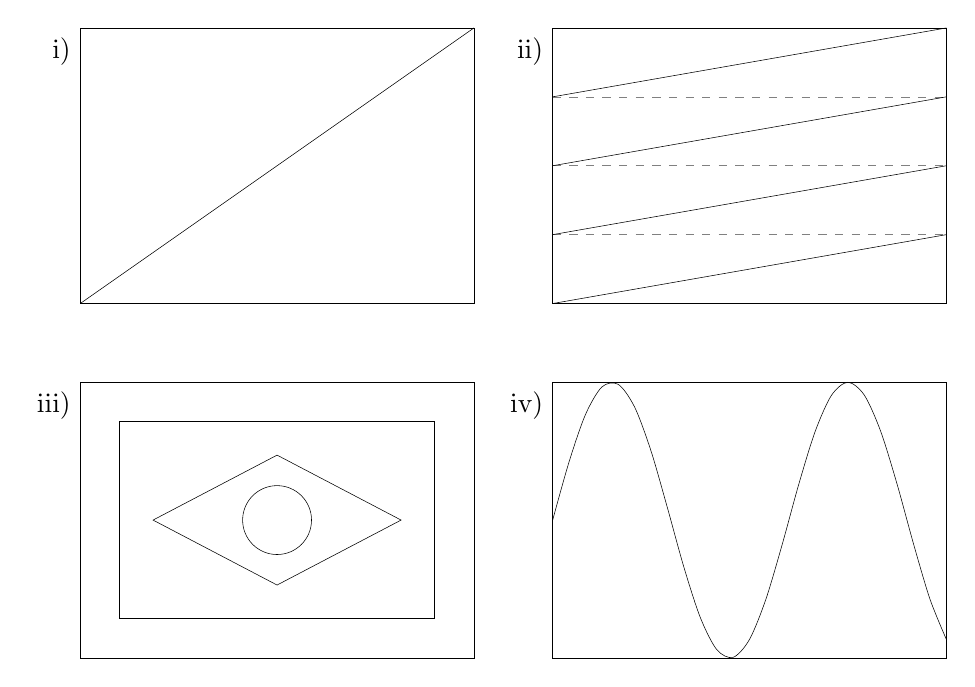
\begin{tikzpicture} [every path/.style={very thin}]
\begin{scope}
\draw (0,0) rectangle (5,3.5) node [below left, xshift=-5 cm,\currentcolor] {i)};;
\draw (0,0) -- (5,3.5);
\end{scope}


\begin{scope} [xshift=6cm]
\draw (0,0) rectangle (5,3.5) node [below left, xshift=-5 cm,\currentcolor] {ii)};
\draw [dashed, help lines] (0,3.5*3/4) -- (5,3.5*3/4); 
\draw (5,3.5) -- (0,3.5*3/4);
\draw [dashed, help lines] (0,3.5*2/4) -- (5,3.5*2/4);
\draw (5,3.5*3/4) -- (0,3.5*2/4);
\draw [dashed, help lines] (0,3.5*1/4) -- (5,3.5*1/4);
\draw (5,3.5*2/4) -- (0,3.5*1/4);
\draw (5,3.5*1/4) -- (0,0);
\end{scope}

\begin{scope} [yshift=-4.5cm]
\draw (0,0) rectangle (5,3.5) node [below left, xshift=-5 cm, \currentcolor] {iii)};;
\draw (.5,.5) rectangle (4.5,3);
\draw (.5+1.7/4,1.75) -- (2.5,.5+1.7/4) -- (4.5-1.7/4,1.75) -- (2.5,3-1.7/4) -- cycle;
\draw (2.5,1.75) circle (0.4375);
\end{scope}

\begin{scope}[xshift =6cm, yshift=-4.5cm]
\draw (0,0) rectangle (5,3.5) node [below left, xshift=-5 cm,\currentcolor] {iv)};;
\draw plot [domain=0:5, smooth] (\x,{1.75*sin (2*pi*\x/3 r)+1.75});
\end{scope}
\end{tikzpicture}
\end{figure}

\end{enumerate}
\end{task}

\begin{task}{cilindro de GNV}



Na Atividade: GNV discutimos a capacidade do tanque de GNV e a compressibilidade do gás nele colocado. Agora vamos aproveitar esta situação para falar do volume ocupado pelo tanque.

\textbf{Parte 1} Aproximação: cota inferior e cota superior

\begin{figure}[H]
\centering

\noindent\includegraphics[width=200bp]{{100}.png}
\end{figure}
\begin{enumerate}
\item {} 
Aproxime o volume ocupado (em metros cúbicos), por um tanque de GNV de capacidade \(15,5m^3\) como o da figura.

\item {} 
Encontre o menor número que você conseguir que seja certamente maior do que o volume ocupado pelo tanque de GNV. Apresente sua resposta em metros cúbicos e em litros. Use os recursos que julgar conveniente.

\item {} 
Agora encontre o maior número que você conseguir que seja certamente menor que o volume ocupado pelo tanque de GNV. Apresente sua resposta em metros cúbicos e em litros. Use os recursos que julgar conveniente.

\item {} 
Encontre o menor número que você conseguir que seja certamente maior que o volume ocupado pelo tanque de GNV. Apresente sua resposta em metros cúbicos e em litros. Novamente você pode usar os recursos que julgar conveniente para resolver a atividade.

\item {} 
Crie um modelo aproximado do tanque usando figuras conhecidas, busque as fórmulas para o cálculo do volume destas figuras e obtenha uma nova aproximação para o volume do tanque.

\item {} 
Discuta o significado da diferença entre as suas aproximações para o volume do tanque e a capacidade especificada pelo vendedor, de \(15,5m^3\).

\end{enumerate}

\textbf{Parte 2}

Dentre os carros populares, os mais econômicos na cidade fazem \(14 km / l\) usando gasolina e \(10 Km / l\) usando etanol como combustível (Veja a edição de 2018 do \href{http://www.inmetro.gov.br/consumidor/pbe/veiculos\_leves\_2018.pdf}{Programa Brasileiro de Etiquetagem Veicular} do INMETRO).
\begin{enumerate}
\item {} 
Verifique se é financeiramente mais vantajoso usar gasolina ou etanol com os preços atuais no seu município. Use o preço médio para este cálculo*.
\begin{itemize}
\item {} 
Os preços atuais do GNV, da Gasolina e do Etanol no seu município estão no \href{http://anp.gov.br/preco/prc/Resumo\_Por\_Municipio\_Index.asp}{Sistema de Levantamento de Preços da ANP}.

\end{itemize}

\item {} 
É corrente entre usuários de carros com motor FLEX utilizar a regra dos 70\% para saber se é mais vantajoso usar etanol ou gasolina (Veja por exemplo: \href{http://www.calculoexato.net/calculadora-flex-gasolina-x-alcool/}{calculadora}). A regra funciona assim: se o preço do etanol for até 70\% do preço da gasolina, deve-se comprar etanol, acima desse percentual deve-se comprar gasolina. É claro que o valor 70\% é aproximado. Explique como ela foi obtida.

\end{enumerate}

Estes mesmos veículos fariam aproximadamente 16 Km / m\(\sp{\text{3}}\) de GNV. Digamos que você saiba que o serviço de instalação pode ser financiado em até 10 vezes de R\$ 420,00 para o seu carro.
\begin{enumerate}
\item {} 
Quantos quilômetros você precisaria rodar em média por dia para que você consiga pagar a instalação com a economia de combustível proveniente do uso do GNV. Use o preço médio para este cálculo?

\item {} 
Os motores dos veículos a base destes combustíveis fósseis, como GNV, gasolina e etanol funcionam a base de combustão. Isto é, consomem oxigênio e liberam gás carbônico e água. Um motor regulado libera aproximadamente 2392 gramas de \(CO_2\) por de gasolina e 2252 gramas de CO\_2 por quilograma de GNV. Qual dos dois combustíveis emite menos CO\_2 por cada quilômetro rodado? Considerando que a densidade do GNV no motor do veículo é de aproximadamente 0,8 Kg / m\(\sp{\text{3}}\).

\end{enumerate}
\end{task}

\begin{task}{aproximando pi}



\textbf{Parte 1}

Existe uma constante muito importante na matemática chamada  \(\pi\) (lê-se pi), que aparece nas fórmulas do comprimento da circunferência, área do círculo, volume da esfera, funções trigonométricas e muitas outras.

O valor dessa constante fundamental na matemática é definido como: a metade do comprimento da circunferência de raio um. Nesta atividade usaremos a fórmula da área do círculo para obter uma aproximação de \(\pi\).

Lembre-se que a fórmula para a área de um círculo de raio \(r\) é  \(\pi.r^2\). Dessa forma, para obter uma aproximação de \(\pi\), basta aproximar a área de um círculo e dividir o resultado obtido por \(r^2\). É o que faremos. Mas como aproximar a área de um círculo? Vamos fazer isso usando a área de figuras já conhecidas.
\begin{enumerate}
\item {} 
Desenhe um círculo em um papel em branco (usando uma forma circular ou um compasso) e meça o seu diâmetro. Feito isso, use uma régua para quadricular o papel com quadrados de tamanho um décimo do diâmetro do círculo, como ilustrado a seguir.

\begin{figure}[H]
\centering

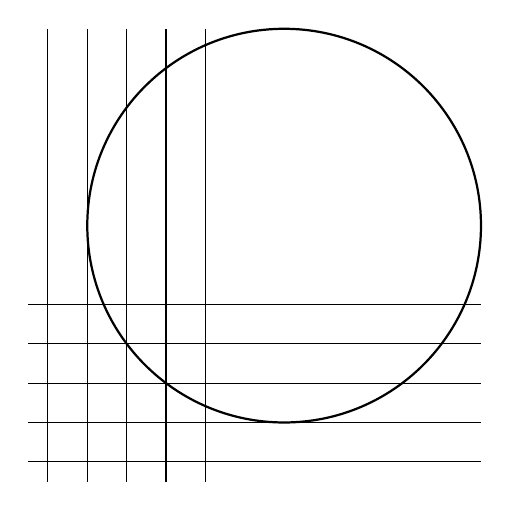
\begin{tikzpicture}[scale=2.5]

\draw [\currentcolor, thick](0,0) circle (1cm);
\foreach \x in {-1.2,-1,-0.8,-0.6,-0.4} \draw (-1.3,\x) -- (1,\x);
\foreach \x in {-1.2,-1,-0.8,-0.6,-0.4} \draw (\x,-1.3) -- (\x,1);

\end{tikzpicture}\end{figure}

\item {} 
Qual a medida da área de um quadradinho do quadriculado que você fez?

\item {} 
Com essa figura, pinte todos os quadradinhos que estão inteiramente contidos no círculo. Qual é a área da região colorida? Agora pinte todos os quadradinhos que têm intersecção não vazia com o círculo. Qual é a área da nova região colorida. Com esses cálculos é possível concluir que a área do círculo está entre que números? Dê uma estimativa para a área do círculo.

\item {} 
Sabendo que a fórmula da área do círculo é \(\pi.r^2\) e usando os cálculos realizados no item anterior, apresente estimativas para \(\pi\), uma menor e outra maior do que o valor de \(\pi\). Algo como: “\(\pi\) é maior do que \_\_\_\_  e menor do que \_\_\_\_”.

\item {} 
Compare os resultados obtidos neste experimento com o valor de \(\pi\) que você conhece.

\item {} 
Que alteração poderia ser feita no processo desse experimento para melhorar a aproximação obtida para \(\pi\)?

\end{enumerate}

\textbf{Parte 2}

A imprecisão do método utilizado na Parte 1 está na limitação do desenho, que, especialmente à medida que os quadradinhos diminuem, dificulta a decisão sobre alguns quadradinhos terem ou não interseção com o círculo. Desta vez, usaremos outro procedimento para aproximar o valor de \(\pi\), sem incorrer neste tipo de imprecisão.
\begin{enumerate}
\item {} 
Calcule o lado do quadrado e do octógono regular inscritos em um círculo de raio um (como na figura abaixo).

\begin{figure}[H]
\centering

\begin{tikzpicture} [scale=3.5, every path/.style={very thick}]


\draw (0,0) circle (1cm);
\draw [color=atento!80] (0.7071,0.7071) -- ++(-90:2*0.7071) -- ++(-180:1.4142) -- ++(-270:1.4142) -- cycle;
\draw [color=destacado!80] (0.7071,0.7071) -- ++(157.5:0.76535) -- ++(202.5:0.76535) -- ++(247.5:0.76535) -- ++(292.5:0.76535) -- ++(337.5:0.76535) -- ++(22.5:0.76535) -- ++(67.5:0.76535) -- cycle;
\draw [color=primario!80] (0.7071,0.7071) -- ++(-56.25:0.39017) -- ++(-56.25-22.5:0.39017) -- ++(-56.25-22.5-22.5:0.39017) -- ++(-56.25-22.5-22.5-22.5:0.39017) -- ++(-56.25-22.5-22.5-22.5-22.5:0.39017) -- ++(-56.25-22.5-22.5-22.5-22.5-22.5:0.39017) -- ++(-56.25-22.5-22.5-22.5-22.5-22.5-22.5:0.39017) -- ++(-56.25-22.5-22.5-22.5-22.5-22.5-22.5-22.5:0.39017) -- ++(-56.25-22.5-22.5-22.5-22.5-22.5-22.5-22.5-22.5:0.39017) -- ++(-56.25-22.5-22.5-22.5-22.5-22.5-22.5-22.5-22.5-22.5:0.39017) -- ++(-56.25-22.5-22.5-22.5-22.5-22.5-22.5-22.5-22.5-22.5-22.5:0.39017)--++(-56.25-22.5-22.5-22.5-22.5-22.5-22.5-22.5-22.5-22.5-22.5-22.5:0.39017)--++(-56.25-22.5-22.5-22.5-22.5-22.5-22.5-22.5-22.5-22.5-22.5-22.5-22.5:0.39017)--++(-56.25-22.5-22.5-22.5-22.5-22.5-22.5-22.5-22.5-22.5-22.5-22.5-22.5-22.5:0.39017)--++(-56.25-22.5-22.5-22.5-22.5-22.5-22.5-22.5-22.5-22.5-22.5-22.5-22.5-22.5-22.5:0.39017)-- cycle;
\foreach  \x in {0,22.5,45,67.5,90,112.5,135,157.5,180,202.5,225,247.5,270,292.5,315,337.5,360} \draw [very thin,help lines] (0,0) -- ++(\x:1);


\end{tikzpicture}

\end{figure}

\item {} 
Calcule a área dessas figuras e use os resultados para estimar o valor de \(\pi\). O valor encontrado é maior ou menor do que \(\pi\)? Compare a aproximação obtida neste item com a obtida na Parte 1 desta atividade. Avalie qualitativamente a melhora da aproximação.

\item {} 
Faça o mesmo agora considerando um hexágono circunscrito ao círculo unitário e estime o valor de \(\pi\) por cima.

\end{enumerate}

Outra forma de estimar el valor de \(\pi\) usando áreas pode ser encontrada no \href{https://www.geogebra.org/m/v2aqzkce}{aplicativo Geogebra: Aproximação de Pi}
\end{task}


\explore{Princípio de Cavalieri}
\label{\detokenize{GE504-8:explorando-principio-de-cavalieri}}\label{\detokenize{GE504-8::doc}}
\begin{task}{Princípio de Cavalieri em 2D}



O Princípio de Cavalieri, objeto de estudo desta seção, apresenta condições para que duas regiões planas (dois sólidos) tenham mesma área ( mesmo volume).
\begin{enumerate}
\item {} 
Use o aplicativo \href{https://ggbm.at/bxrxatwv}{deste link} e o aplicativo \href{https://ggbm.at/gkh7g4y5}{deste link} e tente descrever com as suas palavras o que vem a ser o Princípio de Cavalieri. Registre por escrito a sua descrição.

\item {} 
Use o aplicativo \href{https://ggbm.at/rqpdcc33}{deste link} e veja se a descrição do item anterior ainda serve para este exemplo.

\end{enumerate}
\end{task}

\begin{task}{distância percorrida dada a velocidade instantânea}



A velocidade de um veículo em metros por segundo no intervalo de tempo {[}1,4{]} segundos é dada pela expressão \(v(t) = t^2 - 4t + 5\) cujo gráfico está esboçado na figura.

\begin{figure}[H]
\centering

\begin{tikzpicture}[scale=1.5, every node/.style={scale=1.5}]

\draw [->] (-.1,0) -- (5.5,0) node [above left, scale=0.6] {$t$};
\draw [->] (0,-.1) -- (0,5.5) node [below right, scale=0.6] {$v$};

\foreach \x in {1,...,5} {\draw (\x,.05) -- (\x,-.05)  node [scale=0.5, below] {\x}; \draw (.05,\x) -- (-.05,\x) node [scale=0.5, left] {\x};
}
\node [below left, scale=0.5] at  (-.05,-.05)  {0};

\draw [color=\currentcolor!80, domain=1:4, semithick, smooth] plot  (\x,{(\x)^2 -4*\x+5}) node [color=\currentcolor!80, left, xshift =-0.5cm, yshift=-1cm , scale=0.6] {$v(t)=t^2 - 4t +5$};
\node [ponto, fill=\currentcolor!80, scale=0.7] at (1,2) {} node at (1,2) [above right, scale=0.5] {(1,2)};
\node [ponto, fill=\currentcolor!80, scale=0.7] at (4,5) {} node at (4,5) [above right, scale=0.5] {(4,5)};



\end{tikzpicture}
\end{figure}

\begin{figure}[H]
\centering

\begin{tikzpicture}[scale=1.5, every node/.style={scale=1.5}]

\fill [\currentcolor!50, opacity=0.3, domain =1:4, variable=\x] (1,0) -- plot  (\x,{(\x)^2 -4*\x+5}) -- (4,0) -- cycle;


\draw [->] (-.1,0) -- (5.5,0) node [above left, scale=0.6] {$t$};
\draw [->] (0,-.1) -- (0,5.5) node [below right, scale=0.6] {$v$};

\foreach \x in {1,...,5} {\draw (\x,.05) -- (\x,-.05)  node [scale=0.5, below] {\x}; \draw (.05,\x) -- (-.05,\x) node [scale=0.5, left] {\x};
}
\node [below left, scale=0.5] at  (-.05,-.05)  {0};

\draw [color=\currentcolor!80, domain=1:4, semithick] plot  (\x,{(\x)^2 -4*\x+5}) node [color=\currentcolor!80, left, xshift =-0.5cm, yshift=-1cm , scale=0.6] {$v(t)=t^2 - 4t +5$};
\node [ponto, fill=\currentcolor!80, scale=0.7] at (1,2) {} node at (1,2) [above right, scale=0.5] {(1,2)};
\node [ponto, fill=\currentcolor!80, scale=0.7] at (4,5) {} node at (4,5) [above right, scale=0.5] {(4,5)};


\end{tikzpicture}\end{figure}

É um fato conhecido da física que a distância percorrida pelo veículo entre os instantes \(t = 1\) segundo e \(t = 4\) segundos é dado pela área da região limitada pelo gráfico da função velocidade, pelo eixo \(t\) e pelas retas verticais \(t = 1\) e \(t = 4\) (região hachurada na figura).
\begin{enumerate}
\item {} 
Obtenha um método para aproximar a distância percorrida com erro tão pequeno quanto desejado.

\item {} 
Reveja a atividade anterior e busque argumentar pela validade do Princípio de Cavalieri usando a estratégia adotada no item a) desta atividade.

\end{enumerate}
\end{task}

\begin{task}{volume de concreto de uma barragem}

(Derivada da atividade Staumauer de \href{https://www.geogebra.org/u/lindner}{Andreas Lindner} disponível nos materiais do GeoGebra)



A figura mostra um modelo de barragem que pretende-se construir em concreto. Para isso será necessário conhecer o volume da barragem pronta. O responsável pelo projeto informou que ela tem 92m de comprimento, 24m de altura, que todas as seções transversais são retângulos, que ao pé da parede a largura é de 16m, e no topo é de 4,67m de largura e que a espessura da parede aumenta exponencialmente para cima. Garanta que não faltará concreto para a construção! Melhor sobrar do que faltar.

\begin{figure}[H]
\centering

\noindent\includegraphics[width=400bp]{{105}.png}
\end{figure}
\begin{enumerate}
\item {} 
Obtenha a função que a cada altura z da parede associa a largura da parede naquela altura.

\item {} 
Obtenha uma estimativa inicial para o volume da barragem. A ordem de grandeza basta aqui.

\item {} 
Obtenha uma aproximação melhor que a anterior. Tente fazer de modo que possa ser estabelecido um algoritmo que sirva para o cálculo de aproximações sucessivas.

\end{enumerate}
\end{task}


\arrange{Princípio de Cavalieri}
\label{\detokenize{GE504-9:organizando-as-ideias-principio-de-cavalieri}}\label{\detokenize{GE504-9::doc}}
A imagem apresenta duas retas tracejadas paralelas, um retângulo (à esquerda), um paralelogramos não retângulo ao centro e uma outra figura formada por duas linhas curvas e dois segmentos de reta sobre as retas tracejadas. Em todas elas, se traçarmos uma reta paralela às retas tracejadas obteremos segmentos de comprimento 3cm na região por elas limitada.

\begin{figure}[H]
\centering

\begin{tikzpicture}%[scale=, every node/.style={scale=}]

\draw (0,1) -- (3,1) node [midway, scale=0.8, below] {3};
\draw [xshift=4cm] (0.5,1) -- (3.5,1) node [midway, scale=0.8, below] {3};
\draw [xshift =10cm](0.745,1) -- (3.745,1) node [midway, scale=0.8, below] {3};

\draw [, color=\currentcolor](0,0) rectangle (3,4);
\draw [xshift=4cm, color=\currentcolor] (0,0) -- (3,0) -- (5,4) -- (2,4) -- cycle;
\draw [xshift =10cm, color=\currentcolor] (0,0) -- (3,0) .. controls (4,0.5) and (4,1.5) .. (3,2) .. controls (2,2.5) and (2,3.5) .. (3.5,4) -- (0.5,4) .. controls (-1, 3.5) and (-1, 2.5) .. (0,2) .. controls (1,1.5) and (1,0.5) .. (0,0)
;



\end{tikzpicture}
\end{figure}

As áreas dos dois quadriláteros são iguais pois ambos são paralelogramos de mesma base e mesma altura. Como você já deve imaginar da discussão as atividades iniciais desta seção a área da terceira região também coincide com as duas anteriores. Para esta e outras situações usamos o Princípio de Cavalieri.

\textbf{Princípio de Cavalieri (versão do plano):} Suponha que duas regiões em um plano estão compreendidas entre duas retas paralelas. Se toda reta paralela a essas duas retas intersecta as regiões em segmentos de comprimentos iguais, então as duas regiões têm áreas iguais.

A versão tridimensional é inteiramente análoga, mas trata das áreas das seções e volumes dos sólidos onde a versão plana trata de comprimentos das seções e áreas das regiões.

Todos concordamos que pilhas de formas diferentes formadas com as mesmas peças, têm o mesmo volume. O Princípio de Cavalieri é a situação limite deste argumento quando as alturas das peças tende a zero. \href{https://ggbm.at/kdzfw7xd}{Neste aplicativo} você pode manipular os sólidos e melhorar a sua visualização.

\begin{figure}[H]
\centering

\noindent\includegraphics[width=400bp]{{107}.png}
\end{figure}

\textbf{Princípio de Cavalieri (versão do espaço):} Suponha que dois sólidos no espaço estão compreendidos entre planos paralelos. Se todo plano paralelo a estes dois planos intersectar os sólidos em regiões de áreas iguais, então os dois sólidos têm volumes iguais.

Uma primeira aplicação do Princípio de Cavalieri é o cálculo do volume de cilindro oblíquos. Em um cilindro oblíquo todas as seções por um plano paralelo às bases resultam em regiões congruentes às bases. Por isso, e pelo Princípio de Cavalieri, o volume de qualquer cilindro oblíquo coincide com o volume do cilindro reto de mesma área da base e mesma altura. Portanto, o volume dos cilindros oblíquos também são dados por área da base vezes altura. A figura mostra o caso particular em que este cilindro oblíquo tem base triangular.

\begin{figure}[H]
\centering

\noindent\includegraphics[width=400bp]{{108}.png}
\end{figure}

\textbf{Atenção:} Não confunda a altura do prisma oblíquo com o comprimento de suas arestas laterais.


\practice{}
\label{\detokenize{GE504-10::doc}}\label{\detokenize{GE504-10:praticando}}
\begin{task}{reflexões sobre perímetros e áreas de triângulos}



\textbf{Parte 1}

Na figura, as retas \(r\) e \(s\) são paralelas e os segmentos \(BC\) e \(B'C'\) são congruentes.

\begin{figure}[H]
\centering

\begin{tikzpicture}[scale=1.5, every node/.style={scale=2}]

\draw [fill=\currentcolor!80, color=\currentcolor, opacity=0.4] (1,0) -- (1.75,3) -- (2.5,0) -- cycle;

\draw [fill=\currentcolor!80, color=\currentcolor, opacity=0.4] (3,0) -- (4.75,3) -- (4.5,0) -- cycle;

\foreach \x in {(1,0),(1.75,3),(2.5,0),(3,0),(4.5,0)} \node [ponto] at \x {};

\foreach \x/\y/\z in {(1,0)/B/below,(1.75,3)/A/above, (2.5,0)/C/below,(3,0)/B'/below,(4.5,0)/C'/below} \node  [\z, scale=0.5]  at \x {$\y$};

\node [ponto, color=destacado] at (4.75,3) {} node [color=destacado, above, scale=0.5] at (4.75,3) {$A'$};

\draw (0,0) -- (5,0) node [above right, pos=0, scale=0.5] {$s$};
\draw (0,3) -- (5,3) node [above right, pos=0, scale=0.5] {$r$};

\end{tikzpicture}
\end{figure}
\begin{enumerate}
\item {} 
Qual dos triângulos têm a maior área, \(ABC\) ou \(A'B'C'\)? Explique a sua resposta.

\item {} 
Dentre todos os triângulos que se pode formar movendo A’  sobre a reta \(r\), qual deles tem menor perímetro? Justifique. E o de perímetro máximo?

\end{enumerate}

\textbf{Parte 2}

Seja \(H\) a distância entre as retas \(r\) e \(s\) e considere uma reta \(t\) paralela a \(r\) e a \(s\), que dista \(h\) de \(r\) e intersecta os lados dos triângulos em \(XY\) e \(X'Y'\) como na figura.

\begin{figure}[H]
\centering

\begin{tikzpicture}[scale=1.5, every node/.style={scale=2}]

\draw [fill=\currentcolor!80, color=\currentcolor, opacity=0.4] (1,0) -- (1.75,3) -- (2.5,0) -- cycle;

\draw [fill=\currentcolor!80, color=\currentcolor, opacity=0.4] (3,0) -- (4.75,3) -- (4.5,0) -- cycle;

\foreach \x in {(1,0),(1.75,3),(2.5,0),(3,0),(4.5,0)} \node [ponto] at \x {};

\foreach \x/\y/\z in {(1,0)/B/below,(1.75,3)/A/above, (2.5,0)/C/below,(3,0)/B'/below,(4.5,0)/C'/below} \node  [\z, scale=0.5]  at \x {$\y$};

\node [ponto, color=destacado] at (4.75,3) {} node [color=destacado, above, scale=0.5] at (4.75,3) {$A'$};

\draw (0,0) -- (7,0) node [above right, pos=0, scale=0.5] {$s$};
\draw (0,3) -- (7,3) node [above right, pos=0, scale=0.5] {$r$};

\draw [help lines] (0,2) -- (7,2);
\draw [help lines] (5.5,3) -- (5.5,2) node [midway, right, scale=0.5, black] {$h$};
\draw [help lines] (6.5,3) -- (6.5,0) node [midway, right, scale=0.5, black] {$H$};
\node [ponto, atento, scale=0.7] at (6.5,2) {};

\draw [destacado, thick] (1.5,2) -- (2,2) node [pos=0, ponto] {} node [pos=0, above left, scale=0.5, black] {$X$} node [pos=1, ponto] {} node [pos=1, above right, scale=0.5, black] {$Y$};

\draw [destacado, thick] (4.17,2) -- (4.67,2) node [pos=0, ponto] {} node [pos=0, above left, scale=0.5, black] {$X'$} node [pos=1, ponto] {} node [pos=1, above right, scale=0.5, black] {$Y'$};
\end{tikzpicture}
\end{figure}
\begin{enumerate}
\item {} 
Mostre que, seja lá qual for a distância \(h\), os segmentos \(XY\) e \(X'Y'\) são congruentes.

\item {} 
Seja \(\mathcal{A}\) = Área(\(ABC\)), use o Princípio de Cavalieri para calcular a Área(\(A'B'C'\)).

\item {} 
Calcule Área(\(AXY\)) / Área(\(ABC\)) em termos de \(h\) e de \(H\).

\end{enumerate}
\end{task}

\begin{task}{volume da pirâmide}



\textbf{Parte 1}

O tetraedro de vértice \(V\) e base \(ABC\) da figura possui arestas de comprimentos \(AB\), \(BC\), \(CA\), \(VA\), \(VB\) e \(VC\) respectivamente iguais a 8, 9, 10, 18, 18, 19 cm e altura \(H\) cm. Foi traçado um plano paralelo ao plano \(ABC\) a uma distância \(h\) do ponto \(V\) intersectando o tetraedro no triângulo \(XYZ\) como na figura.

\begin{figure}[H]
\centering

\noindent\includegraphics[width=300bp]{{112}.png}
\end{figure}
\begin{enumerate}
\item {} 
Explique por que o triângulo \(XYZ\) é semelhante ao triângulo \(ABC\) com razão de semelhança \(h / H\).

\item {} 
Calcule a razão Área(\(XYZ\)) / Área(\(ABC\)) em função de \(h\) e \(H\).

\end{enumerate}

\textbf{Parte 2}

Dois tetraedros com áreas iguais em suas bases e alturas iguais têm volume iguais.

Os tetraedros da figura têm bases \(ABC\) e \(A'B'C'\) de mesma área e possuem alturas iguais. Nesta atividade você vai justificar que eles possuem volumes iguais mesmo sem conhecer a fórmula para o volume de um tetraedro.

\begin{figure}[H]
\centering

\noindent\includegraphics[width=300bp]{{113}.png}
\end{figure}
\begin{enumerate}
\item {} 
Assim como na parte anterior, os triângulos \(XYZ\) e \(X'Y'Z'\) são determinados pela interseção do tetraedro original por um plano paralelo aos planos das bases que dista \(h\) dos vértices. Explique por que os triângulos \(XYZ\) e \(X'Y'Z'\) têm áreas iguais.

\item {} 
Use o Princípio de Cavalieri para explicar por que os tetraedros \(V-ABC\) e \(V-A'B'C'\) têm volumes iguais.

\end{enumerate}

\textbf{Parte 3}

Qualquer tetraedro é parte de um prisma triangular formado por outros dois tetraedros de mesmo volume que o tetraedro original.
\begin{enumerate}
\item {} 
Use o aplicativo \href{https://ggbm.at/shmk9dkj}{deste link} para montar o prisma triangular com os três sólidos apresentados.

\item {} 
Como você nomearia estes sólidos dados?

\item {} 
Explique por que os sólidos dados têm mesmo volume (reveja os resultados dos itens anteriores, se necessário).

\end{enumerate}

\textbf{Parte 4}

A sequência de figuras, apresenta uma demonstração sem palavras de um fato matemático.

\begin{figure}[H]
\centering

\noindent\includegraphics[width=430bp]{{114-115---121}.png}
\end{figure}

Portanto,

\begin{figure}[H]
\centering

\noindent\includegraphics[width=400bp]{{122123}.png}
\end{figure}
\begin{enumerate}
\item {} 
Que fato matemático está sendo justificado na sequência de figuras? Em que sentido as igualdades são verdadeiras?

\item {} 
Explique a construção realizada em cada um dos passos. Explique com cuidado especial as “igualdades” entre os tetraedros.

\end{enumerate}
\end{task}

\begin{task}{volume da esfera}



A figura mostra um hemisfério de raio \(r\) (metade de uma bola) e um cilindro de raio e altura iguais a \(r\) de onde foi removido um cone de mesma base e altura que o cilindro (chamaremos este sólido de anticlépsidra).

\begin{figure}[H]
\centering

\noindent\includegraphics[width=200bp]{{124}.png}
\end{figure}
\begin{enumerate}
\item {} 
Descreva a figura formada na seção da bola por um plano que está a uma distância \(h\) do centro.

\item {} 
Descreva a figura formada na seção da anticlépsidra por um plano que está a uma distância \(h\) do plano da base.

\item {} 
As seções têm mesma área?

\item {} 
Explique por que o volume da esfera de raio \(r\) é \(4/3 \pi.r^3\). Você pode usar aqui que o volume do cone é (1/3).(Área da base) x (altura) e que o volume do cilindro é (Área da base) x (altura).

\end{enumerate}
\end{task}


\exercise{}
\label{\detokenize{GE504-E:exercicios}}\label{\detokenize{GE504-E::doc}}\begin{enumerate}
\item {} 
(OBMEP 2018) Alice colocou um litro (1000 \(cm^3\)) de água em uma jarra  e  mediu  o  nível  da  água.  Depois  ela  colocou  um  objeto  maciço  de  prata  na  jarra  e  mediu  novamente  o  nível  da  água, conforme a figura. A massa de um centímetro cúbico de prata é 10,5 gramas. Qual é a massa desse objeto?

\end{enumerate}

\begin{figure}[H]
\centering

\noindent\includegraphics[width=200bp]{{Screenshot_from_2018-12-07_21-01-39}.png}
\end{figure}
\begin{enumerate}
\item {} 
Considere duas garrafas, uma com água e outra com óleo, e dois cubos visualmente idênticos (com as mesmas dimensões), um de aço e outro de chumbo. Ao submergir os cubos, um em cada garrafa, qual líquido desloca mais, a água ou o óleo?

\item {} 
Um copo possui marcas de arroz e de farinha com numerações em níveis diferentes. Porém os números não possuem unidades associadas. Esses números podem corresponder a medidas de volume? E de massa?

\item {} 
Use um copo medida graduado de cozinha para estimar o volume de um ovo. Descreva a sua estratégia, justificando sua validade. Essa experiência também permite estimar a massa do ovo.

\item {} 
Um objeto qualquer que tenha seu volume alterado terá necessariamente também sua massa alterada? Justifique sua resposta.

\item {} 
Um conhecido quebra cabeça é feito a partir de 27 pequenos cubos presos por um fio (Figura x) que podem ser organizados como um único cubo maior (Figura y). Relacione o volume do quebra cabeça nas duas configurações apresentadas: desmontado e montado.

Figura Figura

\item {} 
Um cilindro de gás do tamanho de uma pessoa foi capaz de encher balões suficientes para preencher um cômodo inteiro. Por que não houve conservação de volume?

\item {} 
Fechamos duas garrafas de refrigerante consumidas até a metade por um longo período. Uma delas foi fechada somente colocando a tampa e outra amassando a garrafa antes de tampá-la. Após alguns dias em qual das garrafas o líquido restante perdeu mais gás?

\item {} 
Na feira há duas barracas que vendem feijão de corda. Na primeira barraca vende-se a medida de uma lata vazia de leite condensada por R\$ 2,00. Na segunda o preço de cada medida é de R\$ 3,00, mas neste caso a medida é uma cambuca de plástico. Escolha qual das seguintes estratégias permitiria determinar com precisão o preço de um kilo de feijão em cada barraca.
\#. Comprar R\$ 10,00 em cada barraca e comparar o tamanho das porções.
\#. Comprar uma medida em cada barraca e pesar as porções numa balança e subtrair os resultados.
\#. Comprar uma medida em cada barraca e pesar as porções numa balança e dividir cada resultado pelo preço.
\#. Comprar uma medida em cada barraca, pesar as porções numa balança e dividir o preço pelo peso de cada porção.
Fonte: \url{https://www.directoalpaladar.com.mx/ingredientes-y-alimentos/lo-que-necesitas-saber-del-tofu}

\item {} 
Ligamos para dois fornecedores de feijões e queremos decidir de qual deles compraremos. O primeiro nos fornece o preço medido em termos de garrafas pet de refrigerante. O segundo, contudo nos informa o preço por sacos de feijão. Qual pergunta poderíamos fazer ao segundo fornecedor para tomar a decisão: quantos quilos tem cada saco? ou quantos litros tem cada saco?

\item {} 
A figura a seguir representa um cubo formado por cubos menores. Quantos cubos menores são necessários para formar o cubo da figura?
FIGURA

\item {} 
Qual é a(s) dimensão(ões) relevante para a compra de uma corda? E para a compra de um tecido? E para a compra de gás ou gasolina?

\item {} 
Quantos cubos foram usados para o arranjo tridimensional da figura a seguir?
FIGURA

\item {} 
Uma tinta deve ser aplicada com espessura de 0.1 mm em uma parede retangular de 3m de altura e 6m de largura. Qual a quantidade mínima de tinta que deve ser comprada?

\item {} 
(OBMEP 2017) Vários quadrados foram dispostos um ao lado do outro, em ordem crescente de tamanho, formando uma figura com 100cm de base. O lado do maior quadrado mede 20cm. Qual é o perímetro da figura formada por esses quadrados?

FIGURA

\item {} 
São dadas peças de tamanho 2 por 3 para cobrir um retângulo 5 por 7, como na figura.

FIGURA
\begin{enumerate}
\item {} 
Faça uma figura da cobertura sem sobreposição indicando os cortes necessários em cada peça.

\item {} 
Preencha a tabela com os cortes

\end{enumerate}

\begin{table}[H]
\centering
\begin{tabu} to \textwidth{|c|c|c|c|}
\hline
\thead
Tipo de corte & Área da peça & núm. de peças usadas & área acumulada \\
\hline
figura & & & \\
\hline
figura & & & \\
\hline
figura & & & \\
\hline
figura & & & \\
\hline
\end{tabu}
\end{table}

\item {} 
A partir do desenho da planta de organização de caixas de produtos num estante industrial, a altura da pilha e o número de produtos em cada caixa; deduzir o número total de produtos transportados na estante.

FIGURA

\item {} 
Em quais das figuras a seguir o volume destacado é de \(\frac{1}{2}m^3\)?

\item {} 
Um jogo de blocos de montar possui blocos em forma de paralelepípedos de lados: 2, 4 e 5. Qual é o lado do menor cubo que podemos construir com esses blocos?

\item {} 
Assinale as características mínimas que precisamos conhecer para determinarmos um prisma a menos de congruência.
* altura,
* número de lados do polígono da base,
* área da base,
* uma aresta lateral,
* todas as arestas laterais,
* comprimentos dos lados do polígono da base,
* ângulo entre uma aresta lateral e o plano de uma das bases.
* ângulos internos do polígono da base.
* polígono da base.

\item {} 
Quais dos cilindros a seguir estão determinados a menos de congruência.
\begin{enumerate}
\item {} 
Figura com cilindro circular reto com raio e altura dados.

\item {} 
Figura com cilindro oblíquo com ângulo do eixo com o plano e altura dados.

\item {} 
Figura com cilindro circular reto com área da base e área lateral dados.

\item {} 
Figura com cilindro circular reto com planificação e as dimensões do retângulo formado na planificação.

\item {} 
Figura com cilindro circular oblíquo com raio e comprimento  do eixo dados.

\end{enumerate}

\item {} 
(Enem 2001)  Um fabricante de brinquedos recebeu o projeto de uma caixa que deverá conter cinco pequenos sólidos, colocados na caixa por uma abertura em sua tampa. A figura representa a planificação da caixa, com as medidas dadas em centímetros.

\end{enumerate}